%%%%%%%%%%%%%%%%%%%%%%%%%%%%%%%%%%%%%%%%%
% Masters/Doctoral Thesis 
% LaTeX Template
% Version 2.3 (25/3/16)
%
% This template has been downloaded from:
% http://www.LaTeXTemplates.com
%
% Version 2.x major modifications by:
% Vel (vel@latextemplates.com)
%
% This template is based on a template by:
% Steve Gunn (http://users.ecs.soton.ac.uk/srg/softwaretools/document/templates/)
% Sunil Patel (http://www.sunilpatel.co.uk/thesis-template/)
%
% Template license:
% CC BY-NC-SA 3.0 (http://creativecommons.org/licenses/by-nc-sa/3.0/)
%
%%%%%%%%%%%%%%%%%%%%%%%%%%%%%%%%%%%%%%%%%

%----------------------------------------------------------------------------------------
%	PACKAGES AND OTHER DOCUMENT CONFIGURATIONS
%----------------------------------------------------------------------------------------

\documentclass[
11pt, % The default document font size, options: 10pt, 11pt, 12pt
%oneside, % Two side (alternating margins) for binding by default, uncomment to switch to one side
%chapterinoneline,% Have the chapter title next to the number in one single line
%english, % ngerman for German
spanish,
singlespacing, % Single line spacing, alternatives: onehalfspacing or doublespacing
%draft, % Uncomment to enable draft mode (no pictures, no links, overfull hboxes indicated)
%nolistspacing, % If the document is onehalfspacing or doublespacing, uncomment this to set spacing in lists to single
%liststotoc, % Uncomment to add the list of figures/tables/etc to the table of contents
%toctotoc, % Uncomment to add the main table of contents to the table of contents
parskip, % Uncomment to add space between paragraphs
%nohyperref, % Uncomment to not load the hyperref package
headsepline, % Uncomment to get a line under the header
]{MastersDoctoralThesis} % The class file specifying the document structure



\usepackage[utf8]{inputenc} % Required for inputting international characters
\usepackage[T1]{fontenc} % Output font encoding for international characters

\usepackage{palatino} % Use the Palatino font by default

\usepackage[backend=bibtex,natbib=true, style=numeric, sorting=none]{biblatex} % Use the bibtex backend for bibliography

\addbibresource{references.bib} % The filename of the bibliography

\usepackage[autostyle=true]{csquotes} % Required to generate language-dependent quotes in the bibliography

\usepackage{caption}
\usepackage{subcaption}
\usepackage{todonotes}
\usepackage{multirow}
%------------------------
\usepackage{listings}

%\usepackage[hyphens]{url}
%\usepackage[hidelinks]{hyperref}
%\hypersetup{breaklinks=true}
\urlstyle{same}
%\usepackage{cite}
\hyphenation{biblatex}
%--------------------------

\usepackage{color}

\usepackage{enumitem}
%
%----------------------------------------------------------------------------------------
%	MARGIN SETTINGS
%----------------------------------------------------------------------------------------

\geometry{
	paper=a4paper, % Change to letterpaper for US letter
	inner=2cm, % Inner margin
	outer=3.3cm, % Outer margin
	bindingoffset=2cm, % Binding offset
	top=1.5cm, % Top margin
	bottom=1.5cm, % Bottom margin
	%showframe,% show how the type block is set on the page
}

\usepackage{float}
\usepackage{placeins}

%----------------------------------------------------------------------------------------
%	ESTILO DE LOS BLOQUES DE CODIGO
%----------------------------------------------------------------------------------------

\definecolor{mygreen}{rgb}{0,0.6,0}
\definecolor{mygray}{rgb}{0.5,0.5,0.5}
\definecolor{mymauve}{rgb}{0.58,0,0.82}

\lstdefinelanguage{gherkin} {
	% list of keywords
	keywords={
		Caracter{\'i}stica,
		Caracter\'istica,
		Caracteristica,
		Como,
		Quiero,
		Para,
		Antecedentes,
		Escenario,
		Esquema de escenario,
		Ejemplos,
		Dado,
		Dada,
		Dados,
		Dadas,
		Cuando,
		Entonces,
		Y,
		Pero,
	},
	morekeywords={
		Caracter{\'i}stica,
		Caracter\'istica,
	},
	sensitive=True, % keywords are not case-sensitive
}

\lstset{ %
	backgroundcolor=\color{white},   % choose the background color; you must add \usepackage{color} or \usepackage{xcolor}
	basicstyle=\small\ttfamily,
	breakatwhitespace=false,         % sets if automatic breaks should only happen at whitespace
	breaklines=true,                 % sets automatic line breaking
	captionpos=b,                    % sets the caption-position to bottom
	commentstyle=\color{mygreen},    % comment style
	deletekeywords={...},            % if you want to delete keywords from the given language
	%escapeinside={\%*}{*)},          % if you want to add LaTeX within your code
	%extendedchars=true,              % lets you use non-ASCII characters; for 8-bits encodings only, does not work with UTF-8
	%frame=single,	                   % adds a frame around the code
	keepspaces=true,                 % keeps spaces in text, useful for keeping indentation of code (possibly needs columns=flexible)
	keywordstyle=\color{blue},       % keyword style
	language=[ANSI]C,					% the language of the code
	%otherkeywords={*,...},           % if you want to add more keywords to the set
	numbers=left,                    % where to put the line-numbers; possible values are (none, left, right)
	numbersep=5pt,                   % how far the line-numbers are from the code
	numberstyle=\tiny\color{mygray}, % the style that is used for the line-numbers
	rulecolor=\color{black},         % if not set, the frame-color may be changed on line-breaks within not-black text (e.g. comments (green here))
	showspaces=false,                % show spaces everywhere adding particular underscores; it overrides 'showstringspaces'
	showstringspaces=false,          % underline spaces within strings only
	showtabs=false,                  % show tabs within strings adding particular underscores
	stepnumber=1,                    % the step between two line-numbers. If it's 1, each line will be numbered
	stringstyle=\color{mymauve},     % string literal style
	tabsize=2,	                   % sets default tabsize to 2 spaces
	title=\lstname,                   % show the filename of files included with \lstinputlisting; also try caption instead of title
	morecomment=[s]{/*}{*/},
    inputencoding=utf8,
	extendedchars=true,
	literate=        
		{á}{{\'a}}1 {é}{{\'e}}1 {í}{{\'i}}1 {ó}{{\'o}}1 {ú}{{\'u}}1
		{Á}{{\'A}}1 {É}{{\'E}}1 {Í}{{\'I}}1 {Ó}{{\'O}}1 {Ú}{{\'U}}1
		{à}{{\`a}}1 {è}{{\`e}}1 {ì}{{\`i}}1 {ò}{{\`o}}1 {ù}{{\`u}}1
		{À}{{\`A}}1 {È}{{\'E}}1 {Ì}{{\`I}}1 {Ò}{{\`O}}1 {Ù}{{\`U}}1
		{ä}{{\"a}}1 {ë}{{\"e}}1 {ï}{{\"i}}1 {ö}{{\"o}}1 {ü}{{\"u}}1
		{Ä}{{\"A}}1 {Ë}{{\"E}}1 {Ï}{{\"I}}1 {Ö}{{\"O}}1 {Ü}{{\"U}}1
		{â}{{\^a}}1 {ê}{{\^e}}1 {î}{{\^i}}1 {ô}{{\^o}}1 {û}{{\^u}}1
		{Â}{{\^A}}1 {Ê}{{\^E}}1 {Î}{{\^I}}1 {Ô}{{\^O}}1 {Û}{{\^U}}1
		{œ}{{\oe}}1 {Œ}{{\OE}}1 {æ}{{\ae}}1 {Æ}{{\AE}}1 {ß}{{\ss}}1
		{ű}{{\H{u}}}1 {Ű}{{\H{U}}}1 {ő}{{\H{o}}}1 {Ő}{{\H{O}}}1
		{ç}{{\c c}}1 {Ç}{{\c C}}1 {ø}{{\o}}1 {å}{{\r a}}1 {Å}{{\r A}}1
		{€}{{\EUR}}1 {£}{{\pounds}}1
}

%----------------------------------------------------------------------------------------
%	INFORMACIÓN DE LA MEMORIA
%---------------------------------------------------------------------------------------

\thesistitle{Punku, control de accesos} % El títulos de la memoria, se usa en la carátula y se puede usar el cualquier lugar del documento con el comando \ttitle
\degree{Especialista en Sistemas Embebidos } % Nombre del grado, se usa en la carátula y se puede usar el cualquier lugar del documento con el comando \degreename
\author{Ing. Esteban Daniel Volentini} % Tu nombre, se usa en la carátula y se puede usar el cualquier lugar del documento con el comando \authorname
\supervisor{Ing. Juan Manuel Cruz (FIUBA, UTN-FRBA)} % El nombre del director, se usa en la carátula y se puede usar el cualquier lugar del documento con el comando \supname
\juradoUNO{Esp. Ing. Eric Pernia (FIUBA, UNQ)} % Nombre y pertenencia del un jurado se usa en la carátula y se puede usar el cualquier lugar del documento con el comando \jur1name
\juradoDOS{Esp. Ing. Diego Brengi (INTI)} % Nombre y pertenencia del un jurado se usa en la carátula y se puede usar el cualquier lugar del documento con el comando \jur2name
\juradoTRES{Esp. Ing. Alejandro Permingeat (FIUBA, USAT-Motion)} % Nombre y pertenencia del un jurado se usa en la carátula y se puede usar el cualquier lugar del documento con el comando \jur3name
\fechaINICIO{marzo de 2019}
\fechaFINAL{marzo de 2020}

\subject{Memoria del Trabajo Final de la Carrera de Especialización en Sistemas Embebidos de la UBA} % Your subject area, this is not currently used anywhere in the template, print it elsewhere with \subjectname
\keywords{Sistemas Embebidos, CESE, FIUBA} % Keywords for your thesis, this is not currently used anywhere in the template, print it elsewhere with \keywordnames
\university{Universidad de Buenos Aires} % Your university's name and URL, this is used in the title page and abstract, print it elsewhere with \univname
\faculty{{Facultad de Ingeniería}} % Your faculty's name and URL, this is used in the title page and abstract, print it elsewhere with \facname
\department{Departamento de Electrónica} % Your department's name and URL, this is used in the title page and abstract, print it elsewhere with \deptname
\group{{Laboratorio de Sistemas Embebidos}} % Your research group's name and URL, this is used in the title page, print it elsewhere with \groupname


\hypersetup{pdftitle=\ttitle} % Set the PDF's title to your title
\hypersetup{pdfauthor=\authorname} % Set the PDF's author to your name
\hypersetup{pdfkeywords=\keywordnames} % Set the PDF's keywords to your keywords


\newcaptionname{spanish}{\acknowledgementname}{Agradecimientos}
\newcaptionname{spanish}{\authorshipname}{Declaración de Autoría}
\newcaptionname{spanish}{\abbrevname}{Glosario}
\newcaptionname{spanish}{\byname}{por}

\renewcommand{\lstlistingname}{Algoritmo}% Listing -> Algorithm
\renewcommand{\lstlistlistingname}{Índice de \lstlistingname s}% List of Listings -> List of Algorithms

\renewcommand{\listtablename}{Índice de Tablas}
\renewcommand{\tablename}{Tabla} 

\addtolength{\footnotesep}{2mm} % Espacio adicional en los footnotes

\begin{document}

\frontmatter % Use roman page numbering style (i, ii, iii, iv...) for the pre-content pages

\pagestyle{plain} % Default to the plain heading style until the thesis style is called for the body content

%----------------------------------------------------------------------------------------
%	CARÁTULA
%----------------------------------------------------------------------------------------

\begin{titlepage}
\begin{center}

{\scshape\LARGE UNIVERSIDAD DE BUENOS AIRES\par}\vspace{0.1cm} % University name
{\scshape\LARGE FACULTAD DE INGENIERÍA\par}\vspace{0.1cm} % Faculty name
{\scshape\LARGE Carrera de Especialización en Sistemas Embebidos\par}\vspace{1cm} % Thesis type


\includegraphics[width=.3\textwidth]{./Figures/logoFIUBA.png}
\vspace{1cm}

\textsc{\Large Memoria del Trabajo Final}\\[0.5cm] % Thesis type

{\huge \bfseries \ttitle\par}\vspace{0.4cm} % Thesis title

\vspace{1cm}
\LARGE\textbf{Autor:\\
\authorname}\\ % Author name

\vspace{1cm}

\large
\vspace{10px}
{Director:} \\
{\supname} % Supervisor name
 
\vspace{1cm}
Jurados:\\
\jurunoname\\
\jurdosname\\
\jurtresname
 
\vfill
\textit{Este trabajo fue realizado en la Ciudad de San Miguel de Tucumán, \newline entre \fechaINICIOname \hspace{1px} y \fechaFINALname.}
\end{center}
\end{titlepage}


%----------------------------------------------------------------------------------------
%	RESUMEN - ABSTRACT 
%----------------------------------------------------------------------------------------

\begin{abstract}
\addchaptertocentry{\abstractname} % Add the abstract to the table of contents
%
%The Thesis Abstract is written here (and usually kept to just this page). The page is kept centered vertically so can expand into the blank space above the title too\ldots
\centering

El presente documento describe el desarrollo de Punku, un equipo destinado a controlar el acceso en una puerta utilizando tarjetas de proximidad. Surge por la necesidad de la empresa EQUISER de renovar un equipo existente que hoy resulta obsoleto por los avances de la tecnología. Se espera que el producto desarrollado brinde más funcionalidad con un costo de fabricación menor al del equipo actual.

El proyecto de desarrollo incluyó la especificación de requisitos, la definición de las pruebas de aceptación, el diseño del hardware contemplando la producción en escala y el desarrollo del firmware utilizando un sistema operativo de tiempo real. Para verificar el correcto funcionamiento del equipo se realizaron pruebas unitarias y de integración automatizadas.				

\end{abstract}

%----------------------------------------------------------------------------------------
%	CONTENIDO DE LA MEMORIA  - AGRADECIMIENTOS
%----------------------------------------------------------------------------------------

\begin{acknowledgements}
%\addchaptertocentry{\acknowledgementname} % Descomentando esta línea se puede agregar los agradecimientos al índice
\vspace{1.5cm}

Esta sección es para agradecimientos personales y es totalmente \textbf{OPCIONAL}.  

\end{acknowledgements}

%----------------------------------------------------------------------------------------
%	LISTA DE CONTENIDOS/FIGURAS/TABLAS
%----------------------------------------------------------------------------------------
\renewcommand{\listtablename}{Índice de Tablas}

\tableofcontents % Prints the main table of contents

\listoffigures % Prints the list of figures

\listoftables % Prints the list of tables


%----------------------------------------------------------------------------------------
%	CONTENIDO DE LA MEMORIA  - DEDICATORIA
%----------------------------------------------------------------------------------------

\dedicatory{\textbf{Dedicado a... [OPCIONAL]}}  % escribir acá si se desea una dedicatoria

%----------------------------------------------------------------------------------------
%	CONTENIDO DE LA MEMORIA  - CAPÍTULOS
%----------------------------------------------------------------------------------------

\mainmatter % Begin numeric (1,2,3...) page numbering

\pagestyle{thesis} % Return the page headers back to the "thesis" style

\renewcommand{\tablename}{Tabla} 

% Incluir los capítulos como archivos separados desde la carpeta Chapters
% Descomentar las líneas a medida que se escriben los capítulos

% !TeX encoding = UTF-8
% !TeX spellcheck = es_ES
% Chapter 1

\newcolumntype{L}[1]{>{\raggedright\let\newline\\\arraybackslash\hspace{0pt}}m{#1}}
\newcolumntype{C}[1]{>{\centering\let\newline\\\arraybackslash\hspace{0pt}}m{#1}}
\newcolumntype{R}[1]{>{\raggedleft\let\newline\\\arraybackslash\hspace{0pt}}m{#1}}

\chapter{Introducción General} % Main chapter title

\label{Chapter1}
\label{IntroGeneral}

En el presente capitulo se presentan los aspectos generales del trabajo desarrollado y una breve introducción a las tecnologías utilizadas en el mismo.

\section{Descripción del problema}
\label{sec:descripcion}

El control de las personas que acceden a un ambiente es una de las aplicaciones que se benefician desde hace largo tiempo con los avances de la electrónica. El reemplazo de las cerraduras mecánicas y sus correspondientes llaves por sistemas electrónicos lleva mas de 30 años, y continua en plena expansión. Actualmente existe en el mercado una oferta de equipos muy amplia y variada, que utilizan diferente medios para identificar a las personas que intentan acceder. Los métodos de identificación mas difundidos en la actualidad son:

\begin{itemize}
	\item Clave numérica: para la identificación del usuario se le asigna una clave numérica que se ingresa mediante un teclado que forma parte del equipo. Este esquema es el mas económico pero también el más inseguro ya que la clave puede fácilmente darse a conocer a personas no autorizadas. 
	\item Tarjetas de proximidad: para la identificación se utilizan unos sistemas electrónicos que se alimentan al aproximarlos a un lector y transmiten información que permite identificar al portador. Las tarjetas en realidad pueden adoptar otros formatos como llaveros o etiquetas autoadhesivas. Este esquema resulta más costoso pero también más seguro que el anterior ya que las tarjetas no pueden replicarse fácilmente, aunque si es posible prestarlas a personas no autorizadas.
	\item Reconocimiento de huella digital: para la identificación se toma una imagen de un dedo del usuario y se reconoce la geometría de las huellas digitales del mismo. Este esquema es el mas costos y seguro de todos, ya que duplicar una huella digital es una tarea realmente compleja.
\end{itemize}

Independientemente del medio utilizado para la identificación del usuario, todos los equipos tienen una forma de operación y configuración similar, la que puede ser clasificada en tres grandes grupos:

\begin{itemize}
	\item Equipos autónomos: son los más económicos y fáciles de instalar, ya que solo requieren alimentación y la conexión con el mecanismo que libera la puerta para permitir el acceso. Dentro de este grupo podemos encontrar incluso equipos que se integran dentro de una cerradura tradicional y se alimentan con baterías, lo que simplifica al máximo la instalación de los mismos. La principal desventaja de este tipo de equipos es la gestión de las personas autorizadas a ingresar. En general estos equipos integran unos teclados muy básicos con los que se pueden agregar y borrar las personas autorizadas mediante secuencias de códigos numéricos bastante poco amigables con los usuarios finales.
	\item Equipos en linea: son los mas seguros pero también los mas costos y complejos de instalar. Estos equipos incorporan una interfaz de comunicaciones para validar cada operación de acceso con un servidor central en tiempo real. De esta forma la gestión de las personas autorizadas se realiza en forma centralizada sobre dicho servidor mediante un programa informático mucho mas simple de utilizar. Este esquema puede ademas incorporar mayor complejidad en las validaciones efectuadas para autorizar el ingreso de una persona. La principal desventaja de este esquema es que resulta muy sensible a una falla en la red de comunicaciones o en el servidor de autorizaciones.
	\item Equipos gestionados: son equipos autónomos que incorporan una interfaz de comunicaciones para permitir la gestión de los mismos en una forma más simple. En muchos casos son equipos que pueden ademas operar en linea. Podría pensarse que estos equipo combinan las desventajas de los dos anteriores, pero esto no es verdad. Si bien el costo es mayor que el de un equipo autónomo,  no requiere toda la infraestructura de los equipos que operan en linea, lo que disminuye significativamente el costo total de la solución. A cambio de ese aumento en el costo permiten una gestión mas simple ya que es posible utilizar una computadora con un software amigable.
\end{itemize}

Como se desprende del análisis anterior resulta muy difícil encontrar un equipo adecuado para el mercado hogareño o de pequeñas oficinas. A pesar de que la oferta del mercado es muy amplia no existen mucho equipos que combinen adecuadamente las características de precio con la facilidad de instalación y gestión necesarias en un ambiente donde el usuario final posee conocimientos técnicos muy limitados. Por estas razones la mayoría de los equipos destinados a este mercado corresponden al grupo de los equipos gestionados. Sin embargo la mayoría de los mismos utilizan interfaces de comunicaciones cableadas, las que complican la instalación y permiten la gestión unicamente desde una computadora.

Punku nace como una propuesta de la firma EQUISER para resolver el problema del control de accesos en hogares, pequeñas oficinas, consorcios de departamentos y cocheras. Las características mas importantes de este mercado son la poca cantidad de puertas controladas, falta de personal técnico para la gestión del equipo, y en el caso de los consorcios y cocheras, frecuentes cambios en la lista de personas autorizadas. Para lograr la mejor relación entre seguridad, precio y facilidad de gestión, el equipo puede funcionar con tarjetas de proximidad o con controles remotos. Ademas utiliza una interfaz \emph{Bluetooth} que permite gestionarlo desde un dispositivo móvil, que puede ser una computadora portátil, un teléfono celular inteligente o una tableta. También incorpora una entrada para un sensor que permite detectar la apertura de la puerta, y una salida de alarma para informar cuando la misma permanece abierta por más tiempo del adecuado. En la figura \ref{fig:EquipoActual} se puede ver una imagen del equipo actual con su correspondiente lectora de proximidad.

\begin{figure}[ht]
	\centering
	\vspace{3mm}
	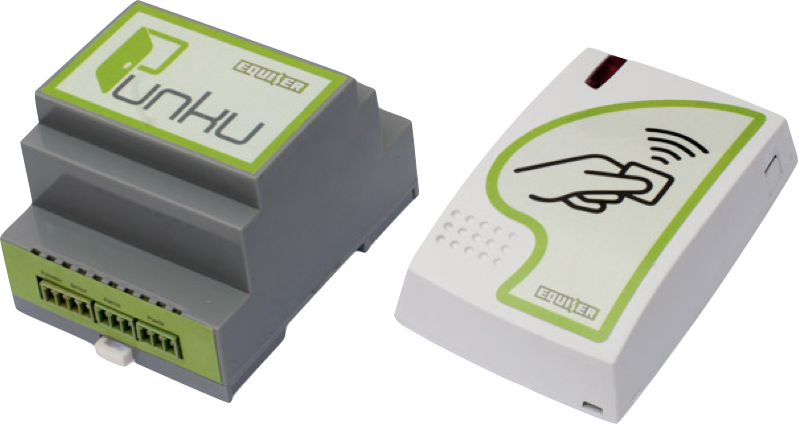
\includegraphics[scale=.5]{./Figures/EquipoActual.png}
	\caption{Fotografía del equipo actual}
	\label{fig:EquipoActual}
\end{figure}

En la tabla \ref{tab:ComparacionActual} se puede ver un cuadro comparativo del producto actual con otros equipos existentes en el mercado. Como se puede observar la oferta se polariza en dos tipos de equipos: totalmente autónomos gestionados mediante un teclado numérico muy limitado o equipos con conexiones cableadas (ethernet o usb) que solo pueden ser gestionados desde computadoras de escritorio o portátiles. En el mercado internacional si existen equipos que se pueden gestionar desde un dispositivo móvil, pero tampoco en este escenario la oferta es abundante. Por estas razones Punku constituye una solución atractiva que busca imponerse principalmente por la facilidad de manejo por parte del usuario final. 

\begin{table}[ht]
	\centering
	\caption{Cuadro comparativo con otros equipos del mercado}
	\begin{tabular}{C{25mm} C{25mm} C{50mm} C{20mm}}    
		\toprule
		\textbf{Equipo}  
			& \textbf{Tecnología} 
			& \textbf{Forma de gestión}
			& \textbf{Valor}  \\
		\midrule
		EQUISER \newline Punku 
			& Proximidad y remotos RF
			& Gestionado desde un \newline celular usando bluetoth
			& \$ 3.000\\
		Tebas \newline 208NW \cite{TEBAS}
			& Proximidad
			& Teclado numérico \newline integrado en el equipo
			& \$ 4.000\\
		ZK \newline MA300IS \cite{ZK}
			& Proximidad \newline y huellas
			& Computadora conectada \newline mediante Ethernet
			& \$ 10.000\\
		ANVIZ \newline T5 Pro \cite{ANVIZ}
			& Proximidad \newline y huellas
			& Computadora conectada \newline mediante Ethernet o USB
			& \$ 8.000\\
		\bottomrule
		
		\hline
	\end{tabular}
	\label{tab:ComparacionActual}
\end{table}

\section{Motivación}
\label{sec:motivacion}

En la figura \ref{fig:BloquesActual} se puede observar un diagrama de bloques del equipo que se produce actualmente. En el mismo encontramos dos unidades funcionales: 

\begin{itemize}
	\item La lectora de proximidad: es la responsable de generar la el campo magnético que alimenta a las tarjetas y decodificar la información enviada por estas.
	\item El procesador: que es el responsable de determinar si la tarjeta leída puede o no acceder, registrar los movimientos de acceso, accionar las salidas para autorizar el ingreso, supervisar el estado de la puerta y comunicarse con el equipo móvil para permitir gestionar la configuración del mismo.
\end{itemize}

\begin{figure}[ht]
	\centering
	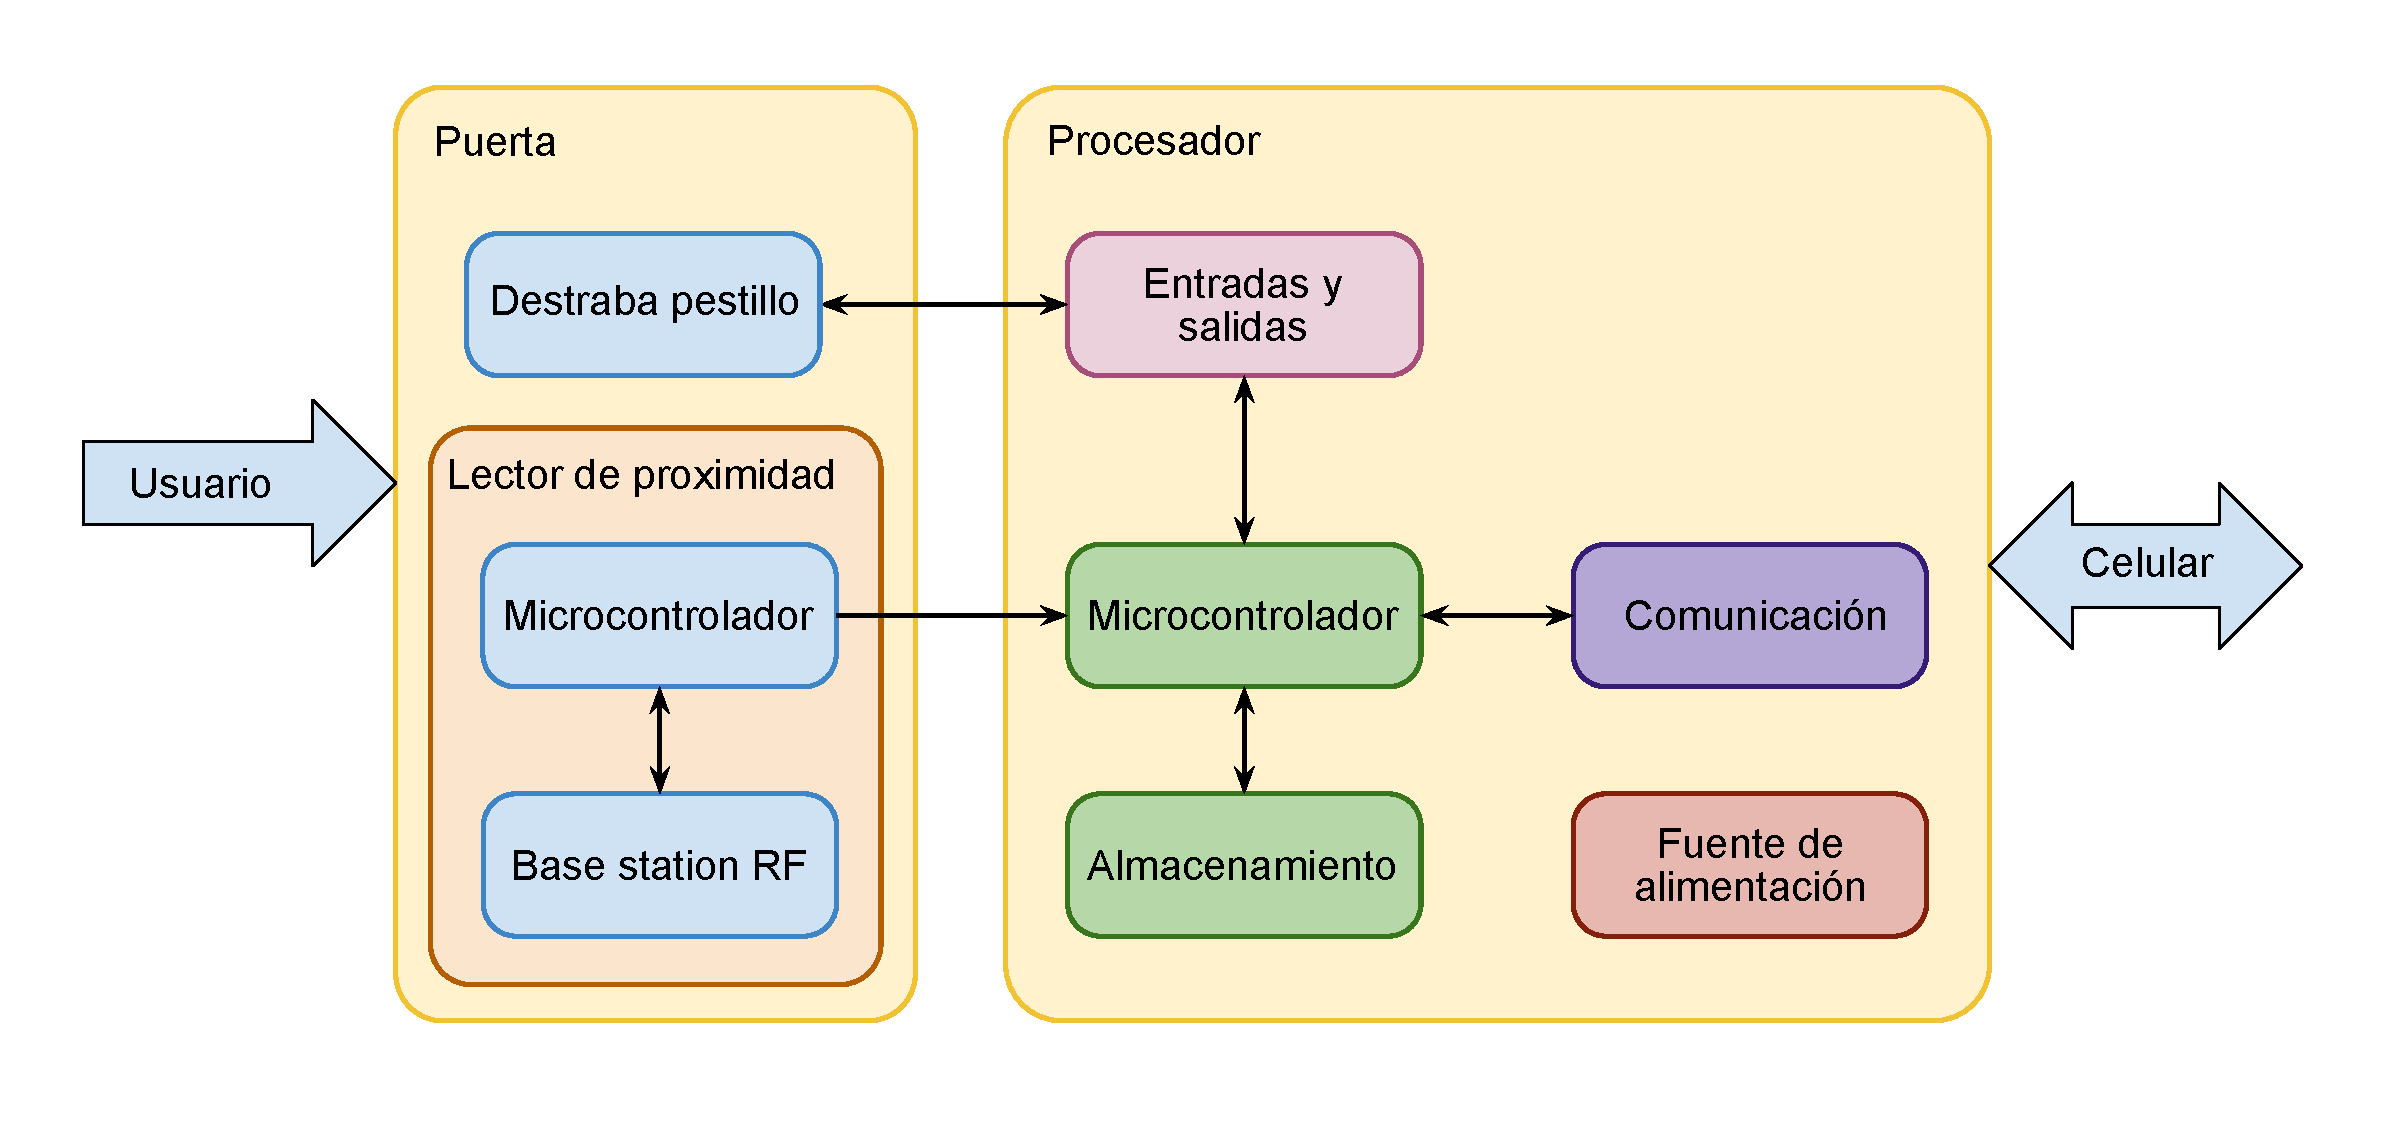
\includegraphics[width=\textwidth]{./Figures/BloquesActual.pdf}
	\caption{Diagrama de bloques del equipo actual}
	\label{fig:BloquesActual}
\end{figure}

La versión en producción del equipo fue diseñada en el año 2013 y los cambios de tecnologías de estos últimos seis años demandaban las siguientes actualizaciones en el diseño del mismo:

\begin{itemize}
	\item Cambio del procesador principal: para el desarrollo original se utilizó un microcontrolador de la familia \emph{ColdFire} producidos por la empresa \emph{Freescale}. Con el avance de los procesadores \emph{Cortex} el fabricante fue dejando de lado el desarrollo de esta gama de productos, por lo que en este momento el microcontrolador utilizado resulta más costoso que un procesador más nuevo con mayores prestaciones. Lamentablemente no existe una oferta por parte del fabricante de un microcontrolador con una disposición de terminales pensada para efectuar un reemplazo directo del utilizado actualmente.
	
	\item Cambio de la interfaz de comunicaciones: el equipo actual utiliza para la comunicación una interfaz \emph{Bluetoth} 2. Poco tiempo después del desarrollo se aprobó la versión 4 de este protocolo, la cual fue adoptado rápidamente por la firma \emph{Apple}. Esta nueva versión del protocolo no es compatible con la anterior, y si bien algunos equipos pueden funcionar en ambos modos de trabajo, este no es el caso de los equipos \emph{iPhone}, donde para privilegiar la duración de la batería solo pueden operar con \emph{Bluetooth} 4.
	
	\item Incorporación de un reloj: al comercializar las primeras unidades surgió el requerimiento de algunos clientes para disponer de un registro de acceso con fecha y hora de cada evento. El equipo actual no dispone de un \emph{Real Time Clock} (RTC) que le permita mantener la fecha y hora cuando el mismo no dispone de alimentación eléctrica. De esta forma si bien el equipo registra los eventos con fecha y hora, la misma vuelve a una fecha inicial preestablecida cada vez que se reinicia el mismo, y es necesaria una comunicación desde el celular para reajustar el reloj interno. El resultado es que la mayoría de los registros de accesos no tienen una fecha y hora validas.
	
	\item Soporte para cerraduras motorizadas: uno de los principales obstáculos para la instalación de equipos para el control de accesos en el mercado al cual esta destinado Punku son los cortes de alimentación eléctrica. Según el tipo de cerradura que se utilice, ante una falla de energía la puerta quedará cerrada y no se podrá acceder, o peor aun quedará abierta en forma permanente. Una solución a este problema es combinar una cerradura con llave y un sistema motorizado que permita la liberación y el bloqueo de la puerta por cualquiera de los medios. Para esto el equipo debe poder invertir la alimentación en la salida que controla al motor, y de esta forma poder liberar o bloquear el mecanismo en función del sentido de giro del mismo.
	
	\item Gestión desde la nube: con el avance en la conectividad a Internet se volvió más común disponer de equipos que pueden ser gestionados en forma remota. En el caso de un control de accesos siempre resulta atractiva la posibilidad de cambiar el permiso de acceso de una persona en forma inmediata sin necesidad de estar cerca del equipo. El uso de \emph{Bluetooth} como interfaz de comunicaciones resulta un obstáculo para esta funcionalidad por su corto alcance y porque nunca se popularizaron equipos equivalente a los \emph{routers} de \emph{WiFi} que permitan el acceso a Internet utilizando Bluetooth.
\end{itemize}

\section{Objetivos y alcance}
\label{sec:objetivos}

El objetivo general del trabajo desarrollado fue el diseño y la implementación de un prototipo de una nueva versión del equipo para control de accesos Punku que resuelva los problemas mencionados en la sección \ref{sec:motivacion}. Los objetivos particulares definidos para el mismo fueron:

\begin{enumerate}
	\item Diseñar el nuevo equipo utilizando un módulo de la familia ESP-32 del fabricante Espressif, el cual incorpora interfaces de comunicación \emph{Wifi} y \emph{Bluetooth} en las versiones 2 y 4.
	
	\item Agregar al nuevo equipo un circuito integrado RTC con respaldo de batería que le permita mantener la fecha y hora validos cuando se producen interrupciones en el suministro de energía eléctrica.
	
	\item Agregar al nuevo equipo la posibilidad de invertir la polaridad de alimentación en la salida que libera la cerradura de forma tal que se pueda utilizar un sistema motorizado para destrabar la puerta.
	
	\item Mantener las características generales del equipo actual en el nuevo diseño, tratando en lo posible de mejorar aun mas la facilidad de gestión del equipo y de disminuir el costo del mismo.
	
	\item Desarrollar el firmware del equipo desde cero, utilizando un sistema operativo de tiempo real y un diseño modular que permita escalar las funcionalidades del equipo.
\end{enumerate}

El resultado esperado es entonces un prototipo totalmente funcional del equipo, que incorpore las mejoras ya mencionadas acompañado de la siguiente documentación:

\begin{enumerate}
	\item Diagrama esquemático del equipo con en el programa KiCad.
	\item Diseño de la placa electrónica realizada en el programa KiCad.
	\item Documento con la especificación de requisitos del firmware según el estandar IEEE-830.
	\item Documento con la arquitectura y el diseño detallado del firmware modelado utilizando diagramas UML.
	\item Documento con las pruebas de aceptación para validar el correcto funcionamiento del equipo escritas en metalenguaje Gherkin. 
	\item Código fuente del firmware para el control del equipo con documentación y comentarios adecuados que faciliten la compresión del mismo.
\end{enumerate}
% !TeX encoding = UTF-8
% !TeX spellcheck = es_ES

\chapter{Introducción Específica}
\label{Chapter2}

En el presente capítulo se abordan en mayor profundidad las distintas tecnologías utilizadas en el equipo. A continuación se detallan los requisitos y casos de uso relevados, junto a las pruebas de aceptación definidas para validar el correcto funcionamiento del prototipo. Por último se presenta en forma abreviada la planificación del proyecto efectuada oportunamente.

\section{Tarjetas de proximidad}
\label{sec:tarjetas}

La identificación por radiofrecuencia o RFID (\emph{Radio Frecuency Identification}) es una tecnología que permite el intercambio de información sin contacto entre un equipo lector y un dispositivo de almacenamiento denominado transpondedor\cite{noauthor_rfid_2020}. También denominados etiquetas RFID, estos dispositivos pueden ser activos si cuentan con alimentación propia, o pasivos si se alimentan del campo electromagnético generado por el equipo lector. 

En el ámbito de los sistemas para el control de accesos, la mayoría de las etiquetas RFID son pasivas y adoptan la forma de una tarjeta plástica, un llavero o una etiqueta autoadhesiva que contiene el chip electrónico junto con la bobina que cumple la función de antena receptora y transmisora. Las distancias de lectura generalmente son del orden de los 10 centímetros, pero pueden extenderse hasta los 15 metros en los sistemas desarrollados para control de vehículos. En el mercado actual de Argentina podemos encontrar, principalmente, cuatro tipos de tarjetas de proximidad:

\begin{itemize}
	\item Tarjetas EM4100: son las más económicas y muy difundidas en el control de accesos. Desarrolladas originalmente por la empresa E\&M Marine\cite{em_microelectronic_em4100_nodate}, fueron ampliamente copiadas por los fabricantes chinos. Estas tarjetas operan con una portadora de 125 KHz, la que modulan en amplitud para transmitir una trama fija de 64 bits, que encapsula un número de serie de 24 bits prefijado durante la fabricación.
	
	\item Tarjetas HID: son el grupo menos difundido en nuestro país, principalmente por el costo y dificultad para adquirirlas. Estas tarjetas operan también con una portadora de 125 KHz, pero la modulan en frecuencia. También transmiten una trama fija que encapsula un número de serie definido en el proceso de fabricación, pero en este caso existen tres variantes de longitud: 24, 36 o 37 bits\cite{hid_global_corporation_hid_nodate}.
	
	\item Tarjetas MIFARE: son las utilizadas por los sistemas de monederos electrónicos y pagos de pasajes en el transporte público de pasajeros. Fueron desarrolladas originalmente por la empresa Philips Semiconductors y hoy son mantenidas por NXP Semiconductors\cite{noauthor_mifare_2019}. Estas tarjetas tienen la capacidad de proteger la memoria utilizando un par de claves criptográficas, de esta manera pueden impedir la lectura o escritura por parte de equipos no autorizados. Se encuentran comprendidas dentro de la norma emitida por la ISO (\emph{Organización Internacional de Normalización}) para regular la operación de tarjetas de proximidad ISO 14443\cite{international_organization_for_standardization_iso_nodate}.
	
	\item Tarjetas UHF: son las utilizadas en los sistemas de telepeaje y para control vehicular, porque pueden alcanzar distancias de lecturas de hasta 15 metros. Estas tarjetas también tienen la capacidad de proteger la memoria utilizando criptografía para impedir la lectura o escritura por parte de equipos no autorizados. Se encuentran normalizadas por la ISO para regular la operación de tarjetas sin contacto de largo alcance en la norma ISO 18000-6C\cite{international_organization_for_standardization_isoiec_nodate}.
\end{itemize}

En la tabla \ref{tab:TarjetasUsadas} se puede observar la comparación entre los distintos tipos de tarjetas de proximidad utilizadas en los sistemas para control de accesos. De estas opciones se decidió que el nuevo equipo opere con el estándar MIFARE, lo que permite utilizar todas las tarjetas de pago electrónico para el transporte público como medio de identificación y acceso, disminuyendo de esta forma la inversión inicial de la instalación.

\begin{table}[ht]
	\centering
	\caption[Tarjetas de proximidad más utilizadas en el control de accesos]{Cuadro comparativo con las tarjetas de proximidad más utilizadas para el control de accesos}
	\begin{tabular}{C{15mm} C{40mm} C{25mm} C{35mm}}
		\toprule
		\textbf{Nombre} 	
			& \textbf{Frecuencia}
			& \textbf{Distancia}	
			& \textbf{Capacidades}
			\\
		\midrule
			EM4100 			
			& 125 KHz / ASK
			& 10 a 15 cm	
			& Solo lectura
			\\
			HID 			
			& 125 KHz / FSK
			& 10 a 15 cm	
			& Solo lectura
			\\
			MIFARE 			
			& 15.56 KHz /ASK
			& 10 a 30 cm	
			& Lectura/Escritura
			\\
			UHF 			
			& 850 a 915 MHz /ASK
			& Hasta 15 m	
			& Lectura/Escritura
			\\
		\bottomrule
		\hline
	\end{tabular}
	\label{tab:TarjetasUsadas}
\end{table}

\section{Aplicaciones para dispositivos móviles}
\label{sec:AplicacionesMoviles}
La elección del modelo de comunicación que se utilizará para la gestión del equipo tiene gran impacto en las herramientas y complejidad de la aplicación del dispositivo móvil. Por eso, aunque el desarrollo de la misma está fuera de los alcances del trabajo, es importante realizar un análisis de las posibles estrategias de implementación.

El mercado de los dispositivos móviles se encuentra polarizado en dos sistemas operativos: Android e iOS. Lamentablemente las herramientas de desarrollo e incluso los lenguajes utilizados por cada plataforma son totalmente incompatibles, esto significa que desarrollar una aplicación que se encuentre disponible para ambas plataformas requiere el doble de esfuerzo. 

Una solución a este problema son las denominadas aplicaciones híbridas\cite{profile_software_services_sl_aplicaciones_nodate}, las cuales en realidad son páginas WEB encapsuladas con el correspondiente navegador de cada plataforma en una aplicación nativa\cite{Frameworks}. Estas aplicaciones se desarrollan entonces en JavaScript y uno de los entornos más difundidos para construir este tipo de aplicaciones es el conjunto Ionic Cordoba\cite{ionic_about_nodate}, el cual permite desarrollar una aplicación para móviles utilizando exclusivamente tecnología WEB. 

Dado que en realidad estas aplicaciones son páginas WEB tienen una serie de restricciones, principalmente en las comunicaciones que pueden realizar y en la interacción con los dispositivos integrados en el equipo móvil, como la cámara de fotos o el micrófono. Algunas de estas restricciones son resueltas utilizando \emph{plugins}, fragmentos de código nativo escrito para cada plataforma que funcionan a modo de adaptador para que la página WEB pueda acceder a estos servicios.

La forma más natural de comunicación para este tipo de aplicaciones es utilizando el protocolo HTTP (\emph{HyperText Transfer Protocol})\cite{noauthor_protocolo_2020}. Este define un conjunto de peticiones, que permiten al cliente efectuar operaciones sobre recursos del servidor\cite{leach_hypertext_nodate}. Originalmente el protocolo HTTP operaba sobre archivos almacenados en el servidor, pero con el tiempo, el concepto de recurso se fue extendiendo. En la actualidad este protocolo se utiliza ampliamente para crear, modificar, consultar y eliminar objetos virtuales como la configuración de un equipo o, en nuestro caso, la lista de personas autorizadas. 

Se denomina API (\emph{Application Programming Interface})\cite{noauthor_interfaz_2019} al conjunto de funciones y procedimientos que una biblioteca pone a disposición para que otro programa puede operar sobre ella. En el caso de este equipo, sería el conjunto de funciones que el firmware pone a disposición de la aplicación móvil para gestionarlo. Esta interfaz se denomina API REST (\emph{REpresentational State Transfer}) cuando se encuentra desarrollada como un conjunto de recursos que pueden ser accedidos utilizando el protocolo HTTP. En estas interfaces la transferencia de información se realiza utilizando el formato JSON(\emph{JavaScript Object Notation})\cite{jsonorg_introduccion_nodate}, que es una forma simple de codificar información en cadenas de texto.

\section{Protocolos inalámbricos}

El aumento del uso de dispositivos móviles con un poder de cómputo cada vez mayor por parte del público abre la puerta a nuevas aplicaciones para estos equipos. En particular para este trabajo, la intención es utilizar un dispositivo móvil como un teléfono inteligente o una tableta, con el fin de gestionar y configurar el equipo para control de accesos. Por esta razón es necesario que la interfaz de comunicaciones implementada sea del tipo inalámbrico, ya que si bien es técnicamente posible utilizar una interfaz USB cableada para conectarse a la mayoría de los teléfonos o tabletas, esta opción no resultaría cómoda ni comercialmente atractiva. En la actualidad existen dos protocolos de comunicación inalámbricos que dominan el mercado:

\begin{itemize}
	\item Bluetooth: es un protocolo diseñado para una red de área personal, con un alcance típico de 10 metros, con bajas tasas de transferencias y optimizado para extender la duración de las baterías\cite{noauthor_bluetooth_2020}. Existen dos versiones principales de este protocolo: la versión 2 y la 4, las cuales no son compatibles entre sí. La mayoría de los dispositivos móviles actuales soportan ambas versiones del protocolo, excepto todos los equipos móviles de la firma Apple, que solo soportan la versión 4 de bajo consumo. En este protocolo la conexión se realiza entre un maestro y un esclavo, y si bien teóricamente se pueden generar redes de dispositivos, en la práctica esto nunca se implementa.
	
	\item WiFi: es un protocolo diseñado para una red de área local, con un alcance típico de 100 metros y altas tasas de transferencias\cite{noauthor_wifi_2020}. Existen varias versiones de este protocolo, las cuales se pueden agrupar en dos familias: las que utilizan una portadora de 2.4 GHz y las de 5 GHz. Las versiones más nuevas pueden utilizar ambas frecuencias simultáneamente para aumentar aún más el ancho de banda. En este protocolo la conexión se realiza generalmente entre un dispositivo y un punto de acceso, que normalmente brinda conexión con una red mayor y eventualmente con Internet.
\end{itemize}

En la tabla \ref{tab:WifiBluetooth} se puede ver un resumen con las características más importantes de las diferentes variantes de ambos protocolos de comunicación. Para el desarrollo del equipo se decidió utilizar WiFi, porque resulta igual de sencillo establecer una conexión punto a punto entre el dispositivo móvil y el equipo que se quiere gestionar, como conectarlo a la red existente en el lugar y gestionarlo desde cualquier ubicación que tenga conexión con dicha red. Incluso es posible, en un futuro, el acceso del equipo a Internet, lo que permitiría su gestión desde cualquier lugar del mundo.

\begin{table}[ht]
	\centering
	\caption[Comparación entre los protocolos Bluetooth y WiFi]{Cuadro comparativo entre las diferentes variantes de los protocolos WiFi y Bluetooth}
	\begin{tabular}{c c c c}
		\toprule
		\textbf{Nombre}	
		& \textbf{Alcance}
		& \textbf{Frecuencia}
		& \textbf{Velocidad}
		\\
		\midrule
		Bluetooth 2.0
		& 10 metros
		& 2,4 GHz
		& 2 MBits/s
		\\
		BLE
		& 10 metros
		& 2,4 GHz
		& 2 MBits/s
		\\
		Wifi 802.11a
		& 100 metros
		& 5 GHz
		& 54 MBits/s
		\\
		Wifi 802.11b
		& 100 metros
		& 2,4 GHz
		& 11 MBits/s
		\\
		Wifi 802.11g
		& 100 metros
		& 2,4 GHz
		& 54 MBits/s
		\\
		Wifi 802.11n
		& 100 metros
		& 2,4 y 5 GHz
		& 600 MBits/s
		\\
		\bottomrule
		\hline
	\end{tabular}
	\label{tab:WifiBluetooth}
\end{table}

La utilización de WiFi resulta más conveniente ya que facilita el uso del conjunto de protocolos TPC/IP y disponer de un servidor HTTP estándar. De esta forma se puede implementar una API REST que, como se explicó en la sección \ref{sec:AplicacionesMoviles}, simplificará la comunicación con aplicaciones híbridas para celulares y páginas WEB. Esta elección también permite que, en un futuro, el equipo se conecte directamente a Internet, y de esta forma gestionarlo desde cualquier lugar del mundo.

\section{Características del equipo}
\label{sec:Caracteristicas}

Dado que el objetivo del trabajo fue el diseño de un equipo comercial, se planteó la necesidad de permitir que pueda adaptarse a diferentes instalaciones. La primera de las opciones de instalación corresponde al tipo de dispositivo que se utiliza para impedir la apertura de la puerta. En este apartado podemos encontrar dos opciones:

\begin{itemize}
	\item Destraba pestillo eléctrico: es un sistema mecánico que actúa como traba para el pestillo de la puerta. Este se libera al energizar una bobina y que por la acción de un resorte vuelve a bloquearse automáticamente cuando se retira la energía eléctrica. De esta forma, mientras el mismo permanece energizado, es posible abrir la puerta.
	
	\item Cerradura electromagnética: es simplemente un electroimán que al ser alimentado ejerce una fuerza que impide la apertura de la puerta. En este caso, la puerta puede abrirse únicamente cuando la cerradura permanece sin alimentación.
	
	\item Cerradura motorizada: en este caso el sistema mecánico de bloqueo es accionado por un motor en lugar de una bobina. Para liberar la puerta es necesario alimentar el motor con una determinada polaridad por un cierto tiempo, o hasta que acciona un sensor que detecta el final del recorrido del mecanismo. La puerta permanece liberada hasta que se alimenta el motor con la polaridad contraria durante un tiempo determinado, o hasta que se acciona un nuevo sensor que detecta el final del recorrido en el sentido contrario al inicial.
\end{itemize}

Como se puede deducir de la descripción anterior, cada tipo de cerradura requiere una señal de control diferente. En particular la mayor diferencia está dada entre los sistemas electromecánicos y los motorizados, debido a la necesidad de una inversión en la alimentación para efectuar el bloqueo de la puerta. 

La otra opción de instalación que podrá definir el usuario final corresponde al uso de un sensor para detectar la apertura de la puerta. En el diseño del equipo se contempla la posibilidad de utilizar este sensor para poder determinar si una persona autorizada ingresa al espacio controlado, y además informar mediante una señal de alarma cuando la puerta permanece abierta más tiempo del adecuado. Un análisis rápido muestra claramente que el comportamiento del equipo debe ser diferente cuando el usuario decide no instalar el sensor para determinar la apertura de la puerta.  

La combinación de las dos opciones antes analizadas determina cuatro modos de funcionamiento principales, los cuales se resumen en la tabla \ref{tab:ModosOperacion}.

\begin{table}[ht]
	\centering
	\caption[Resumen de los modos de funcionamiento del equipo]{Resumen de los modos de funcionamiento del equipo en función la cerradura y la instalación del sensor de puerta.}
	\begin{tabular}{c c L{80mm}}
		\toprule
		\textbf{Cerradura} 	& 
		\textbf{Sensor}	&
		\textbf{Forma de operación} \\
		\midrule
		Electromagnética &
		Sin instalar &
		Se libera la cerradura, cambiando el estado de la alimentación, por un tiempo predefinido. Al finalizar este, se bloquea la cerradura volviendo la alimentación al estado inicial.\\
		\midrule
		Electromagnética &
		Instalado &
		Se libera la cerradura, cambiando el estado de la alimentación, hasta detectar la apertura de la puerta sin exceder un tiempo máximo predefinido. Se supervisa que la puerta no permanezca abierta por más de cierto tiempo.\\
		\midrule
		Motorizada &
		Sin instalar &
		Se libera la cerradura alimentando el motor por un cierto tiempo. Al finalizar el mismo la puerta permanece liberada por un tiempo máximo. Finalmente se bloquea la cerradura alimentando el motor con polaridad inversa durante un cierto tiempo.\\
		\midrule
		Motorizada &
		Instalado &
		Se libera la cerradura alimentando el motor por un cierto tiempo. Al finalizar se supervisa la apertura y cierre de la puerta. Al detectar la apertura de la puerta, o al superar un tiempo máximo de espera, se bloquea nuevamente la cerradura, alimentando el motor con polaridad inversa durante un cierto tiempo.\\
		\bottomrule
		\hline
	\end{tabular}
	\label{tab:ModosOperacion}
\end{table}

\subsection{Requisitos específicos}
\label{sub:Requisitos}

Uno de los primeros puntos que detalla el estándar IEEE-830\cite{institute_of_electrical_and_electronics_engineers_830-1998_nodate}\cite{menendez_especificacion_nodate} para especificación de requisitos son las interfaces externas de la aplicación. Dado que el desarrollo analizado corresponde al firmware de un sistema embebido, las interfaces del software tienen relación directa con las entradas y salidas de la placa electrónica. A continuación se listan los puertos de conexiones que debe implementar el nuevo equipo, incluyendo el identificador asignado a cada uno y una breve descripción del mismo.

\begin{itemize}
	\item PNK-ES001: puerto SPI, utilizado para la comunicación con el circuito integrado del lector RFID.
	\item PNK-ES002: entrada digital opto-aislada, utilizada para conectar el sensor de puerta abierta.
	\item PNK-ES003: salida digital con inversión de polaridad, utilizada para conectar el actuador de la cerradura.
	\item PNK-ES004: entrada digital sin aislación, utilizada para conectar el sensor de cerradura liberada.
	\item PNK-ES005: entrada digital sin aislación, utilizada para conectar el sensor de cerradura bloqueada.
	\item PNK-ES006: entrada digital opto-aislada, utilizada para conectar un pulsador para liberación manual de la puerta.
	\item PNK-ES007: salida digital de contacto seco, utilizada generar una señal de alarma.
	\item PNK-ES008: salida modulada en frecuencia, utilizada para conectar un indicador sonoro para el usuario.
	\item PNK-ES009: salida digital con inversión de polaridad, utilizada para conectar un indicador luminoso para el usuario.
\end{itemize}

Como se explicó en el inicio de la sección \ref{sec:Caracteristicas} uno de los requerimientos importantes del equipo es poder configurar el comportamiento del mismo para adaptarlo a diferentes tipos de instalaciones. Por esta razón se decidió definir claramente cada uno los parámetros de configuración requeridos para lograr la capacidad de personalización deseada. A continuación se listan los parámetros de configuración que debe implementar el nuevo equipo, incluyendo el identificador asignado a cada uno y la descripción formal del mismo.

\begin{itemize}
	\item PNK-PO001: valor numérico en el rango de 100 ms a 2.500 ms, corresponde al tiempo de accionamiento del indicador luminoso PNK-ES009 cuando se produce la lectura de una tarjeta .
	\item PNK-PO002: valor numérico en el rango de 100 ms a 2.500 ms, corresponde al tiempo de accionamiento del indicador sonoro PNK-ES008 cuando se concede el acceso a una tarjeta .
	\item PNK-PO003: valor numérico en el rango de 100 ms a 2.500 ms, corresponde al tiempo de accionamiento del indicador sonoro PNK-ES008 cuando se deniega el acceso a una tarjeta .
	\item PNK-PO004: valor numérico en el rango de 1s a 60s, corresponde al tiempo máximo que la puerta permanece liberada para permitir la apertura de la misma .
	\item PNK-PO005: valor numérico en el rango de 100 ms a 2.500 ms, corresponde al tiempo máximo de accionamiento del motor en cerraduras motorizadas.
	\item PNK-PO006: valor numérico en el rango de 1s a 60s, corresponde al tiempo máximo que la puerta puede permanece abierta antes de generar una señal de alarma.
	\item PNK-PO007: valor lógico que indica si el sensor de puerta abierta se encuentra conectado.
	\item PNK-PO008: valor lógico que indica si el sistema de liberación de la puerta requiere inversión de polaridad.
	\item PNK-PO009: valor lógico que indica si el sistema de liberación de la puerta dispone de sensor para verificar el estado del mismo.
\end{itemize}

Finalmente en lo que respecta a los requisitos funcionales del equipo se los dividió en tres grupos para simplificar la interpretación de los mismos. EL primero corresponde al comportamiento del equipo para el control de acceso, el segundo a las señales de salida que debe generar en función de la configuración y el tercero grupo describe como se realizará la gestión. A continuación se listan los requisitos funciones que debe implementar el nuevo equipo, incluyendo el identificador asignado a cada uno y la descripción formal del mismo.

\begin{itemize}
	\item Requisitos funcionales para el control de accesos
	
	\begin{itemize}
		\item PNK-RS001: el software debe recuperar el número de serie de la tarjeta MIFARE presentada ante el lector.

		\item PNK-RS002: el software debe indicar la lectura de una tarjeta cambiando el color indicador luminoso durante un tiempo PNK-PO001. Para ello debe activar la salida PNK-ES009 con polaridad inversa.

		\item PNK-RS003: el software debe determinar si la tarjeta leída esta incluida en una lista de personas autorizadas y conceder el acceso, o denegarlo si la misma no está incluida.

		\item PNK-RS004: el software debe indicar si se concede el acceso al usuario mediante una melodía de tres tonos ascendentes correspondientes a las frecuencias de 523 Hz, 659 Hz y 784 Hz, todas con una duracción de 100 ms. Para ello debe generar de una señal cuadrada en la interface @ref PNK-ES008 de la frecuencia especificada para cada nota.

		\item PNK-RS005: el software debe indicar si no se concede el acceso al usuario mediante una melodía de tres tonos descendentes correspondientes a las frecuencias de 784 Hz, 659 Hz y 523 Hz, todas con una duracción de 100 ms. Para ello debe generar de una señal cuadrada en la interface @ref PNK-ES008 de la frecuencia especificada para cada nota.

		\item PNK-RS006: cuando concede el acceso a un usuario el software debe accionar el actuador de la puerta para liberarla, esperar la apertura de la puerta o el tiempo máximo de espera fijado por el parámetro PNK-PO004, y al ocurrir cualquiera de los dos eventos debe volver a accionar el actuador de la puerta para bloquearla.

		\item PNK-RS007: cuando un usuario abre la puerta después de un acceso autorizado el software debe supervisar que el cierre de la misma, y si esto no ocurre antes del tiempo máximo de espera fijado por el parámetro PNK-PO006, entonces el software debe generar una señal de alarma hasta que ocurra el cierre de a misma. Para ello debe activar la salida PNK-PO007 en forma permanente hasta que finalice la alarma.

		\item PNK-RS008: el software debe supervisar permanentemente el estado de la puerta para detectar una apertura no autorizada, y debe generar una señal de alarma hasta que ocurra el cierre de a misma. Para ello debe activar la salida PNK-PO007 en forma permanente hasta que finalice la alarma \\
	
		\item PNK-RS009: cuando se activa el pulsador de ingreso conectado a la entrada PNK-ES006 el software debe conceder el acceso siguiendo el mismo comportamiento que para una tarjeta autorizada.

	\end{itemize}

	\item Requisitos funcionales para las señales generadas a los actuadores

	\begin{itemize}
		\item PNK-RS010: si el equipo esta configurado para operar sin sensor de puerta (PNK-PO007 = 0) y con un destraba pestillo eléctrico (PNK-PO008 = 0), cuando se concede el acceso, el software debe activar la salida PNK-ES003 con polaridad directa durante el tiempo máximo de accionamiento de puerta PNK-PO004. Al finalizar este tiempo de espera el software debe apagar la salida PNK-ES003.

		\item PNK-RS011: si el equipo esta configurado para operar con sensor de puerta (PNK-PO007 = 1) y con un destraba pestillo eléctrico (PNK-PO008 = 0), cuando se concede el acceso, el software debe activar la salida PNK-ES003 con polaridad directa hasta que se activa el sensor de puerta abierta PNK-ES002 o hasta que se cumple el tiempo máximo de accionamiento de puerta PNK-PO004. Al finalizar este tiempo de espera el software debe apagar la salida PNK-ES003.
		
		\item PNK-RS012: si el equipo esta configurado para operar sin sensor de puerta (PNK-PO007 = 0), con un motor como actuador (PNK-PO008 = 1) y sin sensores en el mecanismo del motor (PNK-PO008 = 0), cuando se concede el acceso, el software debe activar la salida PNK-ES003 con polaridad directa durante el tiempo máximo de accionamiento del motor PNK-PO005. Al finalizar este tiempo el software debe esperar el tiempo de apertura de la puerta PNK-PO004 y al finalizar el software activar la salida PNK-ES003 con polaridad inversa durante la misma cantidad de tiempo PNK-PO005. Al finalizar este tiempo el software debe apagar la salida PNK-ES003.
		
		\item PNK-RS013: si el equipo esta configurado para operar sin sensor de puerta (PNK-PO007 = 0), con un motor como actuador (PNK-PO008 = 1) y con sensores en el mecanismo del motor (PNK-PO008 = 0), cuando se concede el acceso, el software debe activar la salida PNK-ES003 con polaridad directa hasta que el se activa el sensor PNK-ES004 que indica que el mecanismo está liberado. Después el software debe esperar el tiempo de apertura de la puerta PNK-PO004 y al finalizar el software activar la salida PNK-ES003 con polaridad inversa hasta que se activa el sensor PNK-ES005 que indica que el mecanismo está bloqueado. Al finalizar este tiempo el software debe apagar la salida PNK-ES003. Sí el tiempo que permanece activa la salida PNK-ES003 supera el tiempo máximo PNK-PO004 el software debe apagar la salida y registrar una condición de error.
		
		\item PNK-RS014: si el equipo esta configurado para operar con sensor de puerta (PNK-PO007 = 1), con un motor como actuador (PNK-PO008 = 1) y sin sensores en el mecanismo del motor (PNK-PO008 = 0), cuando se concede el acceso, el software debe activar la salida PNK-ES003 con polaridad directa durante el tiempo máximo de accionamiento del motor PNK-PO005. Al finalizar este tiempo el software debe esperar hasta que se activa el sensor de puerta abierta PKN-ES002 o hasta que se cumple el tiempo máximo de accionamiento de puerta PNK-PO004. Después el software debe activar la salida PNK-ES003 con polaridad inversa durante la misma cantidad de tiempo PNK-PO005. Al finalizar este tiempo el software debe apagar la salida PNK-ES003.
		
		\item PNK-RS015: si el equipo esta configurado para operar con sensor de puerta (PNK-PO007 = 1), con un motor como actuador (PNK-PO008 = 1) y con sensores en el mecanismo del motor (PNK-PO008 = 0), cuando se concede el acceso el software debe activar la salida PNK-ES003 con polaridad directa hasta que el se activa el sensor PNK-ES004 que indica que el mecanismo está liberado. Después el software debe esperar hasta que se activa el sensor de puerta abierta PNK-ES002 o hasta que se cumple el tiempo máximo para la apertura de puerta PNK-PO004. Después el software debe activar la salida PNK-ES003 con polaridad inversa hasta que se activa el sensor PNK-ES005 que indica que el mecanismo está bloqueado. Al finalizar este tiempo el software debe apagar la salida PNK-ES003. Sí el tiempo que permanece activa la salida PNK-ES003 supera el tiempo máximo PNK-PO004 el software debe apagar la salida y registrar una condición de error.
	\end{itemize}			

	\item Requisitos funcionales para la gestión del equipo

	\begin{itemize}
	
		\item PNK-RS016: en cada lectura de tarjeta el software debe registrar en una bitácora la fecha y la hora, el número de la tarjeta leída, si se concedió o no el acceso, si se abrió o no la puerta y si se volvió a cerrar dentro del tiempo establecido.
	
		\item PNK-RS017: en cada acceso por pulsador el software debe registrar en una bitácora la fecha y la hora del acceso, si se abrió o no la puerta, si se volvió a cerrar dentro del tiempo establecido.
	
		\item PNK-RS018: el software debe permitir agregar o eliminar una tarjeta a la lista de personas autorizadas mediante un protocolo de comunicación que utilice la red WiFi como medio de transporte.
	
		\item PNK-RS019: el software debe permitir borrar completamente la lista de personas autorizadas mediante un protocolo de comunicación que utilice la red WiFi como medio de transporte.
	
		\item PNK-RS020: el software debe permitir recuperar todos los eventos de la bitácora, posteriores a una fecha especifica mediante un protocolo de comunicación que utilice la red WiFi como medio de transporte.
	
		\item PNK-RS021: el software debe permitir cambiar los valores de todos los parámetros operativos mediante un protocolo de comunicación que utilice la red WiFi como medio de transporte. 
	\end{itemize}		
\end{itemize}

\subsection{Casos de uso}
\label{sub:CasosDeUso}

Siguiendo las recomendaciones de la ingeniería de software, se documentaron los casos de uso del equipo como parte integral de la especificación de requisitos del software del equipo a desarrollar. En las tablas \ref{tab:CasoPulsador}, \ref{tab:CasoTarjeta}, \ref{tab:CasoConfiguracion}, \ref{tab:CasoAutorizacion} y \ref{tab:CasoBitacora} se detallan los cinco casos de uso identificados durante el análisis de requisitos.

\begin{table}[h!]
	\centering
	\caption{Caso de uso acceso por pulsador}
	\begin{tabular}{L{28mm} L{100mm}}
		\toprule
		\textbf{Titulo} &
		\textbf{Descripción} \\
		\midrule
		Identificador &
		PKN-CU001 \\
		Nombre &
		Acceso por pulsador \\ 
		Descripción	&
		Acceso de una persona utilizando un pulsador \\
		Actor principal &
		Usuario \\
		Disparadores &
		El usuario presiona el pulsador de salida \\
		\multirow[t]{9}{*}{Flujo básico} 
			& 1. El usuario presiona el pulsador de salida \\
			& 2. El software informa que concederá el acceso emitiendo un sonido corto y agudo \\
			& 3. El software acciona el mecanismo para permitir la apertura de la puerta \\
			& 4. El software espera el tiempo accionamiento de cerradura PNK-PO004 \\
			& 5. El usuario abre la puerta antes de que se complete el tiempo de cerradura \\
			& 6. El software acciona el mecanismo para impedir una nueva apertura de la puerta \\
			& 7. El software espera el tiempo de puerta abierta PNK-PO006 \\
			& 8. El usuario cierra la puerta antes de que se complete el tiempo de puerta abierta \\
			& 9. El software registra el acceso en la bitácora de novedades \\
		\multirow[t]{3}{*}[5mm]{Flujo alternativo} 
			& 5. El usuario no abre la puerta antes de que se complete el tiempo PNK-PO004 \\
			& 5.1. El software acciona el mecanismo para impedir una nueva apertura de la puerta \\
			& 5.2. El software registra en la bitácora de novedades que el usuario no ingresó \\
		\multirow[t]{6}{*}[5mm]{Flujo alternativo} 
			& 8. El usuario no cierra la puerta antes de que se complete el tiempo PNK-PO006 \\
			& 8.1. El software informa el error de puerta abierta con un sonido continuo \\
			& 8.2. El software espera el cierre de la puerta \\
			& 8.3. El usuario cierra la puerta \\
			& 8.4. El software deja de emitir el sonido \\
			& 8.5. El software registra en la bitácora de novedades que el usuario dejó la puerta abierta \\
		Precondiciones &
		La puerta debe estar cerrada \\
		Postcondiciones &
		La puerta debe estar cerrada \\
		\bottomrule
		\hline
	\end{tabular}
	\label{tab:CasoPulsador}
\end{table}

\begin{table}[h!]
	\centering
	\caption{Caso de uso acceso por tarjeta de proximidad}
	\begin{tabular}{L{28mm} L{100mm}}
		\toprule
		\textbf{Titulo} &
		\textbf{Descripción} \\
		\midrule
		Identificador &
		PKN-CU002 \\
		Nombre &
		Acceso por tarjeta \\ 
		Descripción	&
		Acceso de una persona autorizada utilizando una tarjeta de proximidad \\
		Actor principal &
		Usuario con tarjeta de proximidad \\
		Disparadores &
		El usuario presenta la tarjeta delante del lector \\
		\multirow[t]{9}{*}{Flujo básico}
			& 1. El usuario presenta la tarjeta delante del lector \\
			& 2. El software verifica que la tarjeta leída esta incluida en la lista de tarjetas autorizadas \\
			& 3. El software informa que concederá el acceso emitiendo un sonido corto y agudo \\
			& 4. El software acciona el mecanismo para permitir la apertura de la puerta \\
			& 5. El software espera el tiempo accionamiento de cerradura PNK-PO004 \\
			& 6. El usuario abre la puerta antes de que se complete el tiempo de cerradura \\
			& 7. El software acciona el mecanismo para impedir una nueva apertura de la puerta \\
			& 8. El software espera el tiempo de puerta abierta PNK-PO006 \\
			& 9. El usuario cierra la puerta antes de que se complete el tiempo de puerta abierta \\
			& 10. El software registra el acceso en la bitácora de novedades \\
		\multirow[t]{3}{*}[5mm]{Flujo alternativo} 
			& 2. El software determina que la tarjeta leída no está incluida en la lista de tarjetas autorizadas \\
			& 2.1. El software informa que no concederá acceso emitiendo un sonido largo y grave \\
			& 2.2. El software registra en la bitácora de novedades que no se concedió el acceso al usuario \\
		\multirow[t]{3}{*}[5mm]{Flujo alternativo} 
			& 6. El usuario no abre la puerta antes de que se complete el tiempo PNK-PO004 \\
			& 6.1. El software acciona el mecanismo para impedir una nueva apertura de la puerta \\
			& 6.2. El software registra en la bitácora de novedades que el usuario no ingresó \\
		\multirow[t]{6}{*}[5mm]{Flujo alternativo} 
			& 9. El usuario no cierra la puerta antes de que se complete el tiempo PNK-PO006 \\
			& 9.1. El software informa el error de puerta abierta con un sonido continuo \\
			& 9.2. El software espera el cierre de la puerta \\
			& 9.3. El usuario cierra la puerta \\
			& 9.4. El software deja de emitir el sonido \\
			& 9.5. El software registra en la bitácora de novedades que el usuario dejó la puerta abierta \\
		Precondiciones &
		La puerta debe estar cerrada \\
		Postcondiciones &
		La puerta debe estar cerrada \\
		\bottomrule
		\hline
	\end{tabular}
	\label{tab:CasoTarjeta}
\end{table}

\begin{table}[h!]
	\centering
	\caption{Caso de uso configuración del equipo}
	\begin{tabular}{L{28mm} L{100mm}}
		\toprule
		\textbf{Titulo} &
		\textbf{Descripción} \\
		\midrule
		Identificador &
		PKN-CU003 \\
		Nombre &
		Configuración del equipo \\ 
		Descripción	&
		Configuración del equipo desde un teléfono celular o una computadora \\
		Actor principal &
		Software de gestión \\
		Disparadores &
		Recepción de un comando de configuración \\
		\multirow[t]{5}{*}[2mm]{Flujo básico} 
			& 1. El software recibe un comando para actualizar la configuración \\
			& 2. El software recibe los nuevos parámetros de configuración \\
			& 3. El software valida los nuevos parámetros de configuración \\
			& 4. El software aplica los nuevos parámetros de configuración \\
			& 5. El software envía una confirmación informando que los parámetros se aplicaron correctamente \\
		\multirow[t]{2}{*}[5mm]{Flujo alternativo} 
			& 3. Los parámetros recibidos son incorrectos \\
			& 3.1. El software envía una notificación de error informando que los parámetros son incorrectos \\
		Precondiciones &
		Ninguna \\
		Postcondiciones &
		Ninguna \\
		\bottomrule
		\hline
	\end{tabular}
	\label{tab:CasoConfiguracion}
\end{table}

\begin{table}[h!]
	\centering
	\caption{Caso de uso gestión de las personas autorizadas}
	\begin{tabular}{L{28mm} L{100mm}}
		\toprule
		\textbf{Titulo} &
		\textbf{Descripción} \\
		\midrule
		Identificador &
		PKN-CU004 \\
		Nombre &
		Gestión de las personas autorizadas \\ 
		Descripción	&
		Configuración de la lista de tarjetas autorizadas desde un teléfono celular o una computadora \\
		Actor principal &
		Software de gestión \\
		Disparadores &
		Recepción de un comando para actualización de la lista de tarjetas autorizadas \\
		\multirow[t]{5}{*}[2mm]{Flujo básico} 
			& 1. El software recibe un comando para actualizar la lista de tarjetas autorizadas \\
			& 2. El software recibe la nueva lista de tarjetas autorizadas \\
			& 3. El software valida la lista de tarjetas autorizadas recibida \\
			& 4. El software reemplaza la lista de tarjetas autorizadas actual por la recibida \\
			& 5. El software envía una confirmación informando que se actualizó la lista de tarjetas autorizadas \\
		\multirow[t]{2}{*}[5mm]{Flujo alternativo} 
			& 3. La lista de tarjetas autorizadas no es válida \\
			& 3.1. El software envía una notificación de error informando que la lista de tarjetas no es válida \\
		Precondiciones &
		Ninguna \\
		Postcondiciones &
		Ninguna \\
		\bottomrule
		\hline
	\end{tabular}
	\label{tab:CasoAutorizacion}
\end{table}

\FloatBarrier

\begin{table}[h!]
	\centering
	\caption{Caso de uso consulta de la bitácora de accesos}
	\begin{tabular}{L{28mm} L{100mm}}
		\toprule
		\textbf{Titulo} &
		\textbf{Descripción} \\
		\midrule
		Identificador &
		PKN-CU005 \\
		Nombre &
		Acceso a la bitácora del equipo \\ 
		Descripción	&
		Consulta de la bitácora del equipo desde un teléfono celular o una computadora \\
		Actor principal &
		Software de gestión \\
		Disparadores &
		Recepción de un comando de consulta de la bitácora \\
		\multirow[t]{2}{*}{Flujo básico} 
			& 1. El software recibe un comando para recuperar la bitácora de novedades \\
			& 2. El software envía la bitácora de eventos \\
		Flujo alternativo &
		Ninguno \\
		Precondiciones &
		Ninguna \\
		Postcondiciones &
		Ninguna \\
		\bottomrule
		\hline
	\end{tabular}
	\label{tab:CasoBitacora}
\end{table}


\subsection{Pruebas de aceptación}
\label{sub:PruebasAceptacion}

El último paso de la especificación de requisitos consistió en la definición de las pruebas de aceptación del equipo, las que servirán para validar el cumplimiento de los requisitos ya listados. Para formalizar las pruebas se siguieron los lineamientos definidos por la metodología BDD (\emph{Behaviour Driven Development})\cite{smart_bdd_2015} para el desarrollo de software. Esta propone utilizar un metalenguaje denominado Gherkin para escribir las pruebas en forma de un guión en lenguaje natural, de forma tal que puedan ser validadas por el cliente. Para organizar la estructura de este, el lenguaje define los siguientes elementos:

\begin{itemize}
	\item Característica: corresponde al conjunto de pruebas para validar un comportamiento especifico del equipo. Cada archivo de pruebas contiene una sola característica que se nombra con una frase corta. A continuación se debe detallar quién pide esa característica, qué acciones espera poder realizar y qué beneficio le otorga. Cada característica está formada por un conjunto de escenarios que definen las pruebas necesarias para validarla. 
	\item Escenario: corresponde a cada una de las pruebas que se efectúan para validar una característica en particular. El escenario se nombra con una frase corta que lo describa y está formado por una serie de sentencias que comienzan con las palabras dado, cuando y entonces. Existe también la posibilidad de agrupar escenarios similares utilizado una tabla de ejemplos y definiendo el esquema de una prueba que se repite para cada ejemplo de la tabla.
	\item Dado: corresponde a las sentencias que definen los condiciones iniciales para poder ejecutar la prueba descrita en el escenario. Normalmente se utilizan al principio del guion.
	\item Cuando: corresponde a las sentencias que definen las acciones que se efectúan para completar la prueba.
	\item Entonces: corresponde a las sentencias que describen el comportamiento esperado del equipo como resultado de efectuar una acción sobre él.
\end{itemize}

A continuación se detallan las pruebas de aceptación definidas para el equipo siguiendo la metodología propuesta.

\vspace{4mm}

\lstinputlisting[firstline=5,language=gherkin,caption=Prueba de aceptación para la validar la apertura por pulsador.]{Features/pulsador.feature}

\vspace{8mm}

\lstinputlisting[firstline=5,language=gherkin,caption=Prueba de aceptación para la validar la apertura por tarjeta de proximidad.]{Features/tarjeta.feature}

\newpage

\lstinputlisting[firstline=5,language=gherkin,caption=Prueba de aceptación para la validar la detección de puerta abierta.]{Features/alarma.feature}

\lstinputlisting[firstline=5,language=gherkin,caption=Prueba de aceptación para la validar la gestion de tarjetas autorizadas.]{Features/autorizacion.feature}

\newpage

\lstinputlisting[firstline=5,language=gherkin,caption=Prueba de aceptación para la validar el registro de los eventos de acceso y alarma.]{Features/bitacora.feature}

 
\chapter{Diseño e Implementación} % Main chapter title
\label{Chapter3} 

En este capítulo se presentan y fundamentan las decisiones adoptadas durante el diseño del equipo, la implementación de la placa electrónica y el desarrollo del firmware.

\section{Diseño del hardware}
\label{sec:hardware}

Un aspecto muy importante que se tuvo en cuenta desde el momento mismo de seleccionar los componentes que se utilizaron en el diseño del equipo es la realidad del medio en el que fabricará y comercializará el producto. EQUISER es una microempresa que comercializa actualmente, en promedio, dos unidades al mes. Esto determina que la fabricación se efectúe en lotes de entre diez y veinte unidades, que representan cantidades muy pequeñas para el estándar de la industria electrónica. Si bien la firma tiene capacidad para importar componentes del exterior, los constantes cambios en las políticas aduaneras del país y la incidencia del costo de los fletes en compras pequeñas llevaron a  minimizar la dependencia de proveedores extranjeros.

En este contexto, y como una solución de compromiso entre la disponibilidad local, la facilidad de montaje, el costo y las prestaciones, se adoptó como procesador principal del equipo el módulo ESP-WROOM-32D de la empresa Espressif. Basado en un procesador de doble núcleo Xtensa de 32bits, que puede operar con una frecuencia de hasta 240 MHz, este microcontrolador dispone de 520 kB de memoria RAM interna y se integra en el módulo 4 MB de memoria flash. Implementa entradas y salidas tanto digitales como analógicas, y puertos de comunicaciones con los protocolos SPI, I2C y UART. Para la comunicación inalámbrica están disponibles una interfaz Bluetooth que puede funcionar con las versiones 2 y 4 del protocolo, y una interfaz WiFi que opera en 2.4 GHz que cumple con las variantes b, g y n del estándar IEEE802.11.

Este módulo se presenta como el sucesor del ESP8266, un diseño pensado originalmente como interfaz WiFi de bajo costo para pequeños microcontroladores, que ganó una cuota importante del mercado cuando el fabricante puso a disposición del público las herramientas para desarrollar versiones propias del firmware. Esto permitió integrar la aplicación directamente dentro del módulo y convertirlo de esta forma en el procesador principal del sistema. Uno de los factores clave del éxito de esta propuesta es el costo y la relativa facilidad de montaje del módulo, características que se mantienen en el ESP-WROM-32D, la versión seleccionada para este diseño. 

En la figura \ref{fig:DiagramaBloques} se presenta el diagrama de bloques del nuevo equipo. Si se lo compara con el de la figura \ref{fig:BloquesActual}, que corresponde al diseño original del equipo, podemos observar las siguientes diferencias:

\begin{figure}[ht]
	\centering
	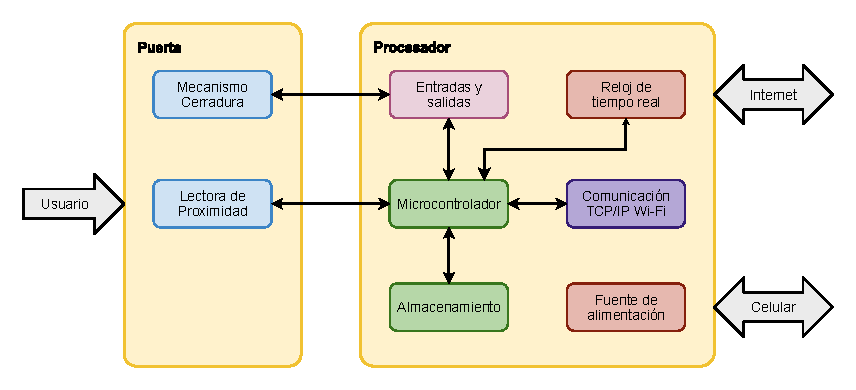
\includegraphics[width=\textwidth]{Figures/BloquesNuevo.pdf}
	\caption{Diagrama de bloques del equipo desarrollado}
	\label{fig:DiagramaBloques}
\end{figure}

\begin{itemize}
	\item Se unificaron las dos unidades funcionales del equipo anterior en el procesador. Así, quedó instalada en la puerta únicamente la placa electrónica que implementa la antena de RFID con el circuito integrado responsable de la generación del campo electromagnético y el procesamiento analógico de la señal recibida. Esto permite además de reducir la cantidad de componentes y centralizar en el firmware principal todo el procesamiento de la comunicación con la tarjeta de proximidad.
	\item En el bloque de entradas y salidas se cambió la conexión con el sistema de cerradura para  controlar indistintamente sistemas electromagnéticos o motorizados. Asimismo se agregaron sensores de fin de carrera para el mecanismo de la cerradura, lo que además de aumentar la confiabilidad del sistema permite prolongar la vida útil de los componentes al evitar esfuerzos innecesarios.
	\item Se cambió el bloque de comunicaciones Bluetooth por una interfaz WiFi, lo que permitió además adoptar el protocolo TPC/IP para la comunicación con el equipo. Esta interfaz puede operar en modo punto de acceso, lo que permite efectuar una comunicación punto a punto con el celular de la misma forma que se hacía con el Bluetooth. Pero también puede operar en modo estación, de esta forma el equipo puede conectarse una red WiFi existente y permitir la gestión desde cualquier dispositivo autorizado que tenga conexión con esta red.
	\item Se incorpora un reloj de tiempo real independiente del procesador que será el responsable de mantener la fecha y hora del sistema. Este bloque incluye una batería de respaldo que le permite continuar funcionando cuando el equipo no cuenta con alimentación.
\end{itemize}

\section{Prototipo del hardware}
\label{sec:prototipo}

En el diseño de la placa electrónica se siguieron los mismos criterios que ya se mencionaron en la sección \ref{sec:hardware} para la selección de los componentes. Se decidió mantener el gabinete actual, lo que determinó la geometría de la placa y la posición de la mayoría de los conectores. Se decidió también que la placa se realizaría con las capacidades de fabricación del único fabricante de circuitos impresos de la provincia, a quien se le encomendaría la producción del primer prototipo. Con estas restricciones el circuito impreso debía resolverse en dos capas y en un área de 87 x 66 mm. 

El trazado de las pistas de cobre no resultó simple, ya que como puede observarse en la figura \ref{fig:Componentes} una parte importante del área de la placa se encuentra ocupada por componentes, lo que sumado a la restricción de utilizar pistas de 0,5 mm y vías de 1 mm impuesta por el proceso de fabricación aumentó la dificultad del proceso de diseño. 

\begin{figure}[ht]
	\centering
	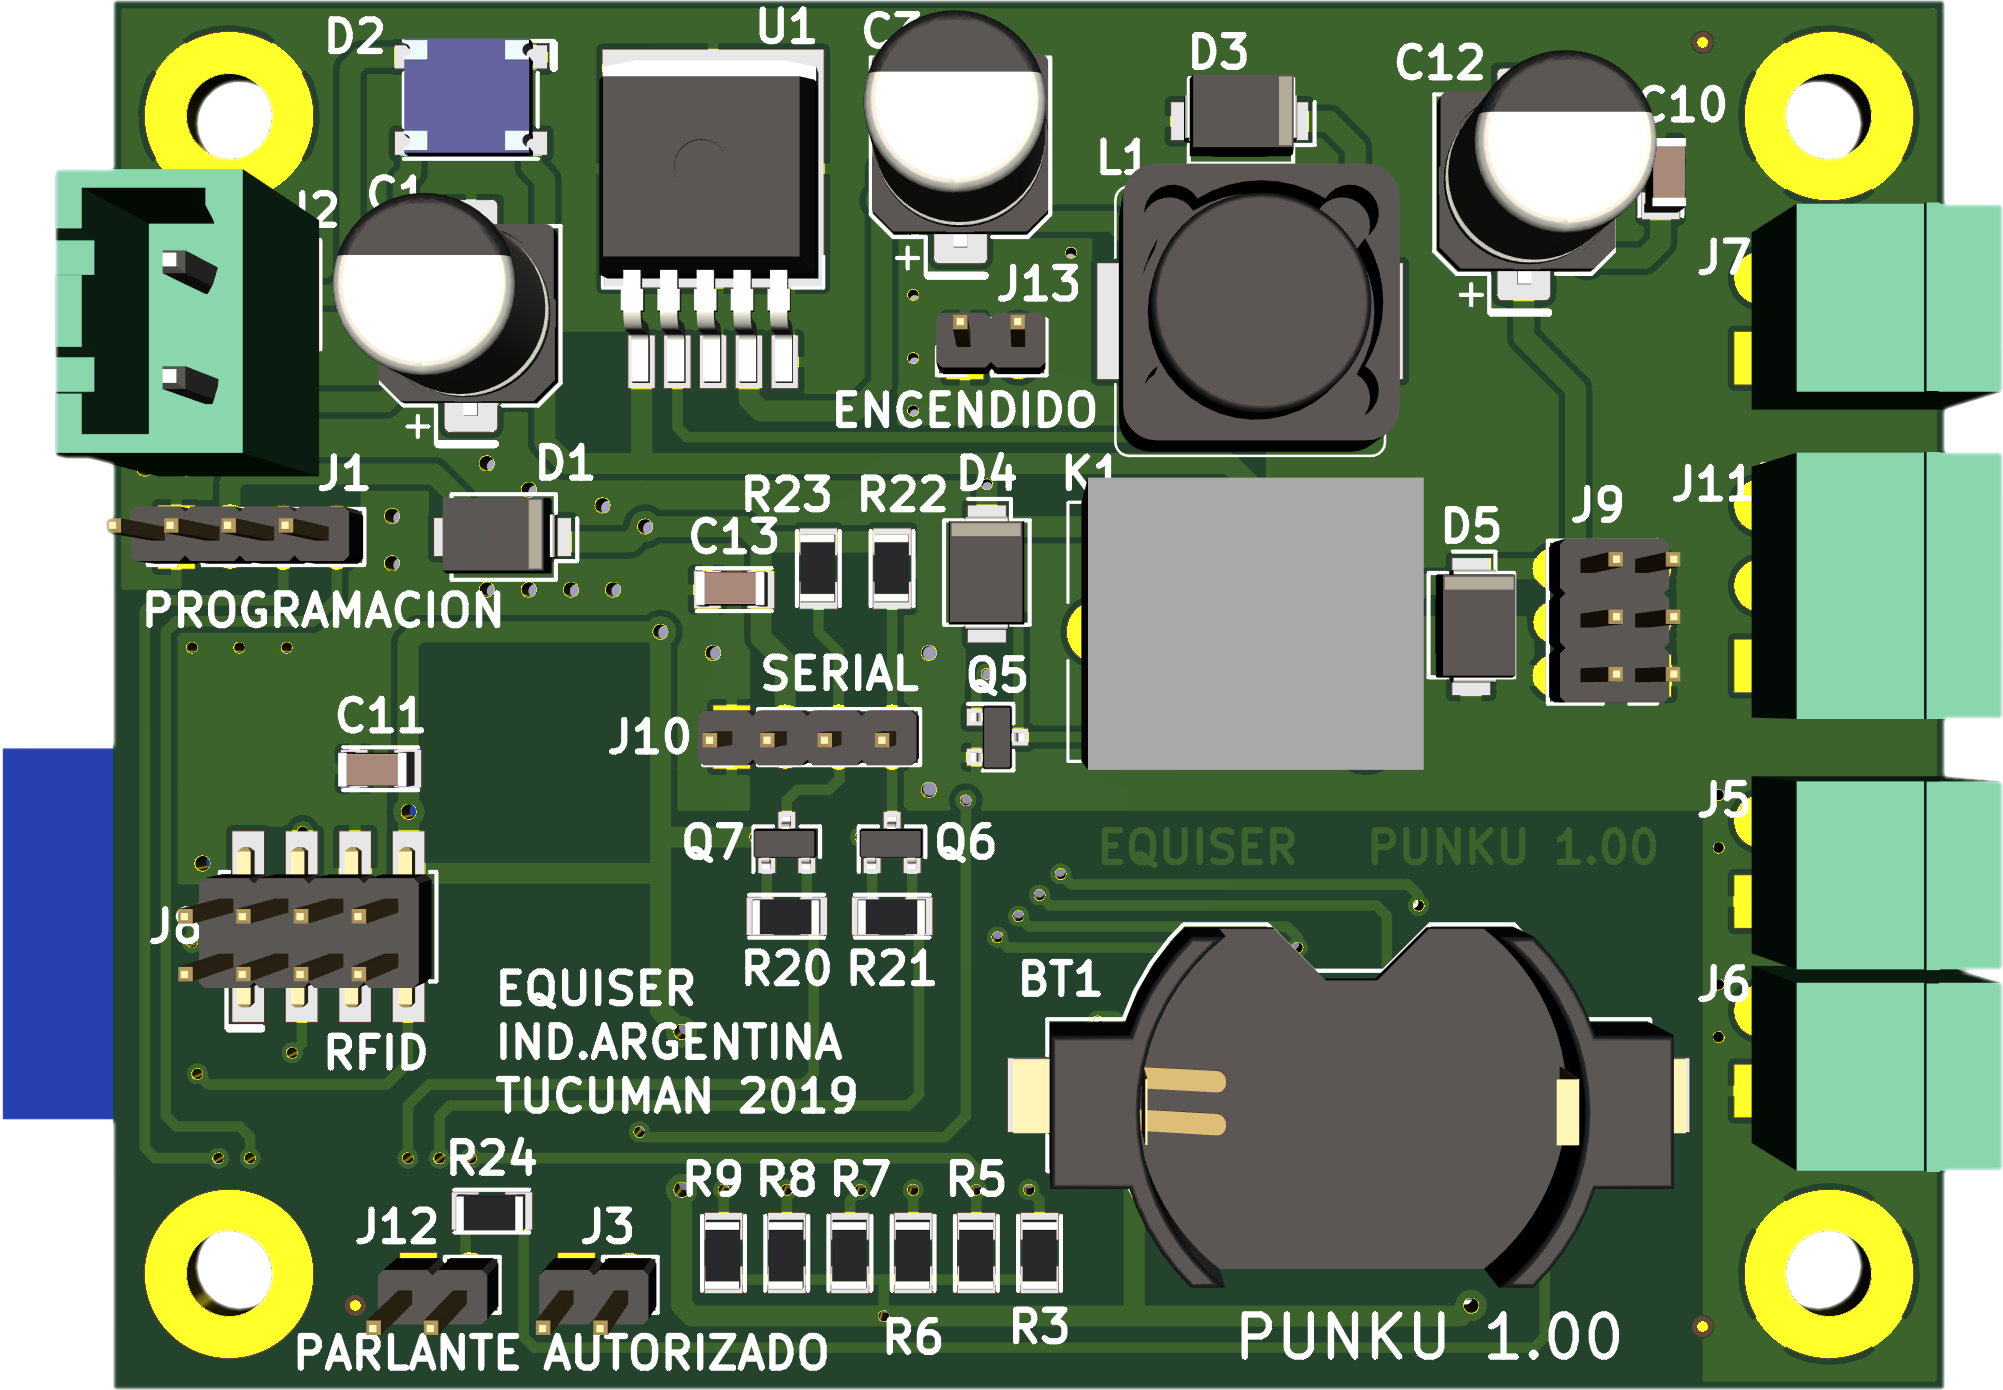
\includegraphics[width=0.9\textwidth]{Figures/ModeloPlaca.png}
	\caption[Modelo tridimensional de la placa electrónica]{Modelo tridimensional de la placa electrónica.}
	\label{fig:Componentes}
\end{figure}

Se efectuó un proceso de doble revisión sobre el diagrama esquemático del circuito y el diseño de la placa, y se incorporó una serie de recomendaciones efectuadas por los revisores como la utilización de los planos de tierra en las zonas de la placa generadoras de ruido electromagnético. Además de los controles mencionados, fue necesario un tercera revisión para detectar y corregir los últimos errores antes de la fabricación de la placa.

La construcción del prototipo se efectuó en forma manual, y durante el proceso se detectaron dificultades para el montaje en algunos componentes, originados en la separación entre los planos de masa y las pistas de señales. En el diseño se adoptó un valor similar al de separación entre pistas, pero debido a la falta de precisión en la máscara antisoldante que puede observarse en la imagen \ref{fig:ProblemasMascara}, este valor resultó pequeño. Durante el proceso de soldadura se generaron puentes de estaño entre los terminales de los componentes y el plano de masa circundante.

\begin{figure}[ht]
	\centering
	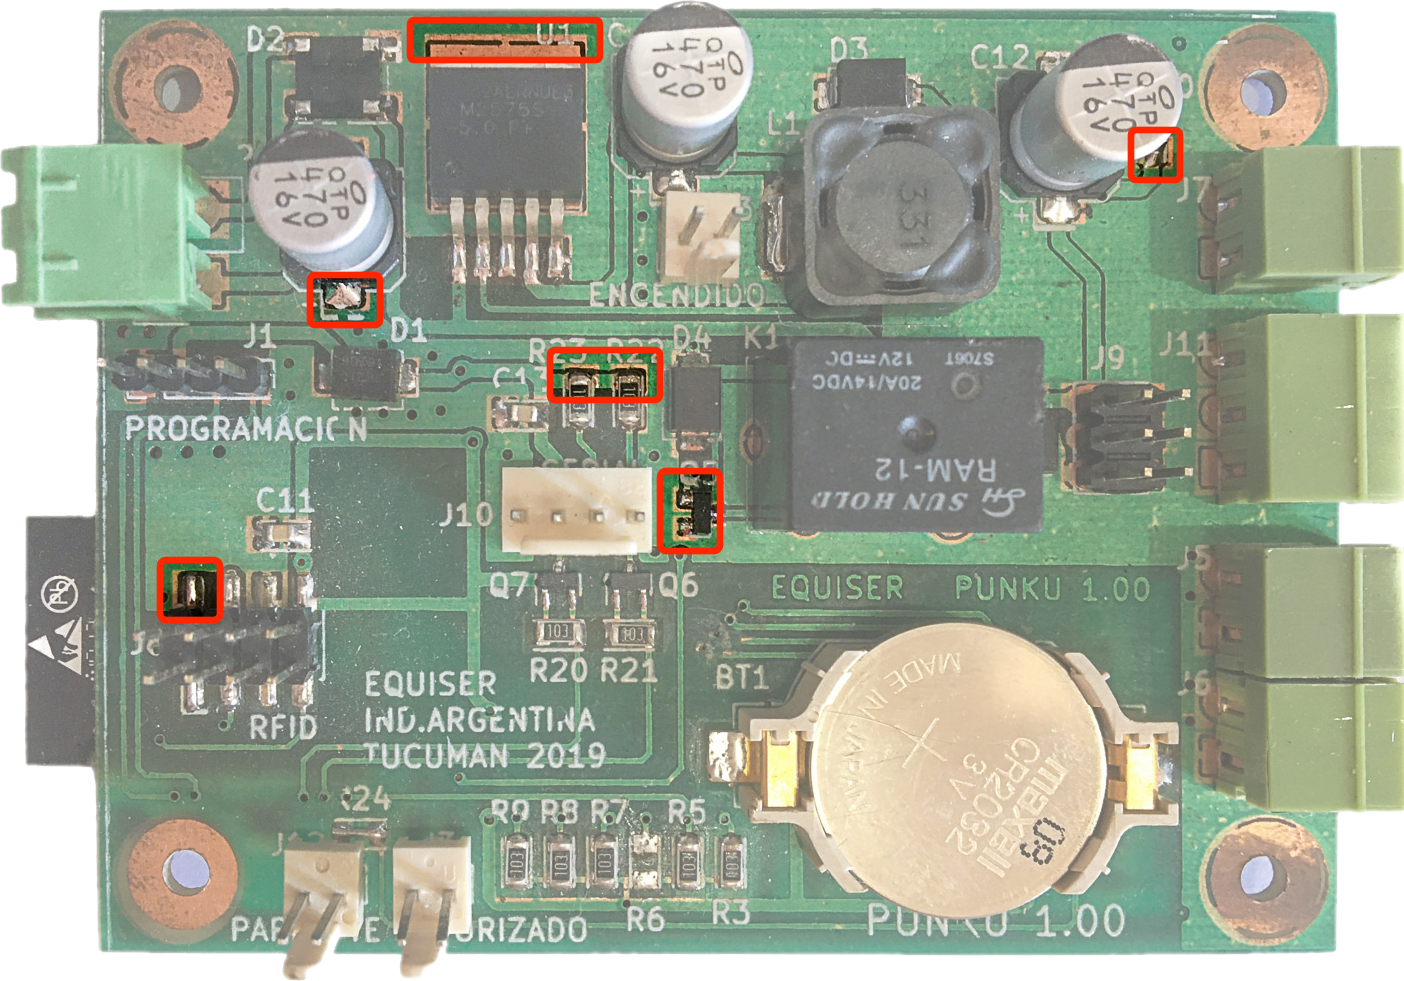
\includegraphics[width=0.9\textwidth]{Figures/LadoComponentes.png}
	\caption[Problemas con la  máscara antisoldante del prototipo]{Imagen que muestra la falta de precisión en la aplicación de la máscara antisoldante del prototipo.}
	\label{fig:ProblemasMascara}
\end{figure}

Para resolver este problema se removieron varios componentes del prototipo, y se recurrió al uso de abundantes cantidades \emph{flux} para volver a soldarlos evitando los cortocircuitos. Este proceso demandó mucho más tiempo de montaje, por lo que también se corrigió el diseño de la placa para aumentar el valor de guarda en los planos de masa, y evitar este problema en las siguientes placas. \todo{revisar}

\section{Diseño del firmware}
\label{sec:firmware}

\subsection{Arquitectura del firmware}
\label{sub:Arquitectura}

Uno de los objetivos planteados para el trabajo en la sección \ref{sec:objetivos} fue la reingeniería completa del firmware del equipo, que permitiera incorporar el uso de un sistema operativo de tiempo real y el reuso de los componentes comunes en otros proyectos similares. Para esto se decidió utilizar una arquitectura de capas, que se puede observar en el diagrama de componentes de la figura \ref{fig:DiagramaComponentes}. En la misma se pueden identificar claramente cuatro capas:

\begin{itemize}
	\item ESP-IDF: corresponde al conjunto de funciones provistas por el fabricante para facilitar el desarrollo en la plataforma. Allí se incluyen los controladores para los puertos GPIO, SPI, I2C y PWM. También se incluye la implementación del sistema de archivos FAT para tarjetas SD y de un servidor HTTP completo.

	\item Plataforma: implementa una capa de abstracción del hardware, también conocida como HAL (\emph{Hardware Abstraction Layer}), que permite independizar el resto del código desarrollado de la plataforma provista por el fabricante. Esta capa facilita la reutilización del resto de los componentes en proyectos similares y la eventual migración del firmware a otra plataforma.

	\item Controladores: implementa una serie de clases que se pueden reutilizar en otros proyectos fácilmente ya que no dependen del hardware ni de la aplicación.

	\item Aplicación: implementa la lógica propia del equipo mediante un conjunto de tareas que ejecutan concurrentemente en un sistema operativo de tiempo real.
\end{itemize}


\begin{figure}[ht]
	\centering
	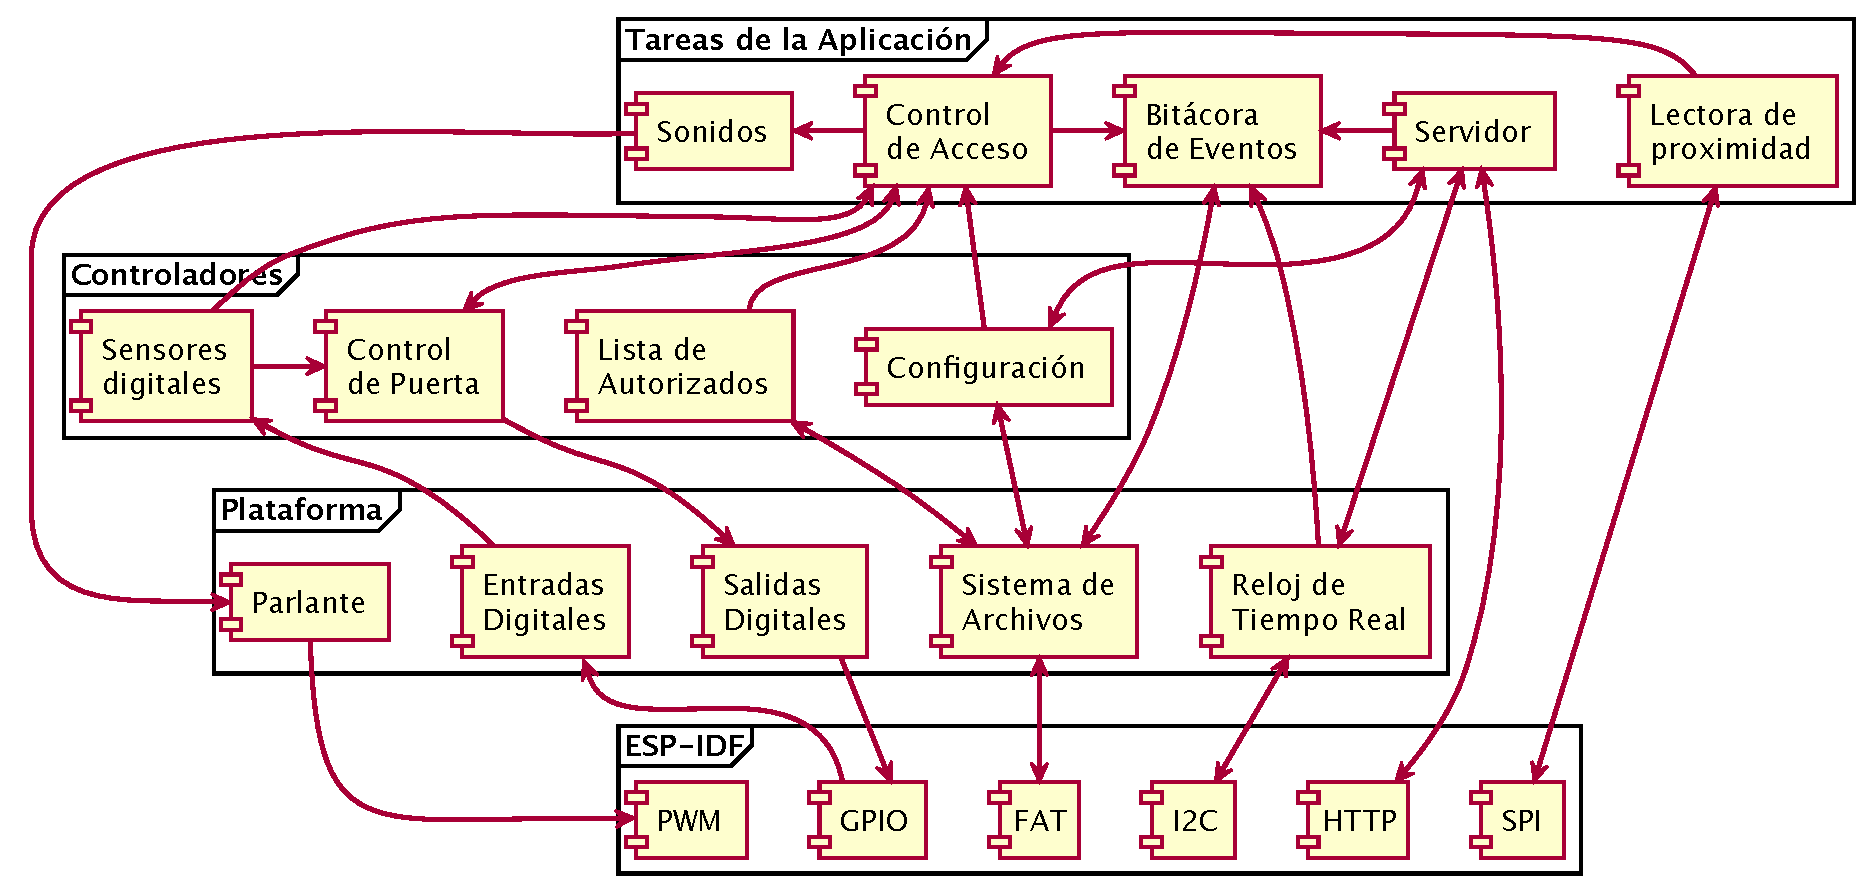
\includegraphics[width=\textwidth]{./Figures/PNK-DC001.pdf}
	\caption[Diagrama de componentes del firmware del equipo]{Diagrama de componentes del firmware del equipo.}
	\label{fig:DiagramaComponentes}
\end{figure}

Para el modelado de los componentes se utilizó el análisis orientado a objetos, lo que arrojó como resultado una colección de clases con sus respectivos métodos y atributos. Una imagen completa de este diseño se puede observar en el diagrama de clases que se muestra en la figura \ref{fig:DiagramaClases}. Allí solo están incluidos los componentes de las tres clases superiores desarrolladas en el marco del trabajo. En las siguientes subsecciones se explican brevemente las responsabilidades asignadas a cada una de estas clases.

\begin{figure}[H]
	\centering
	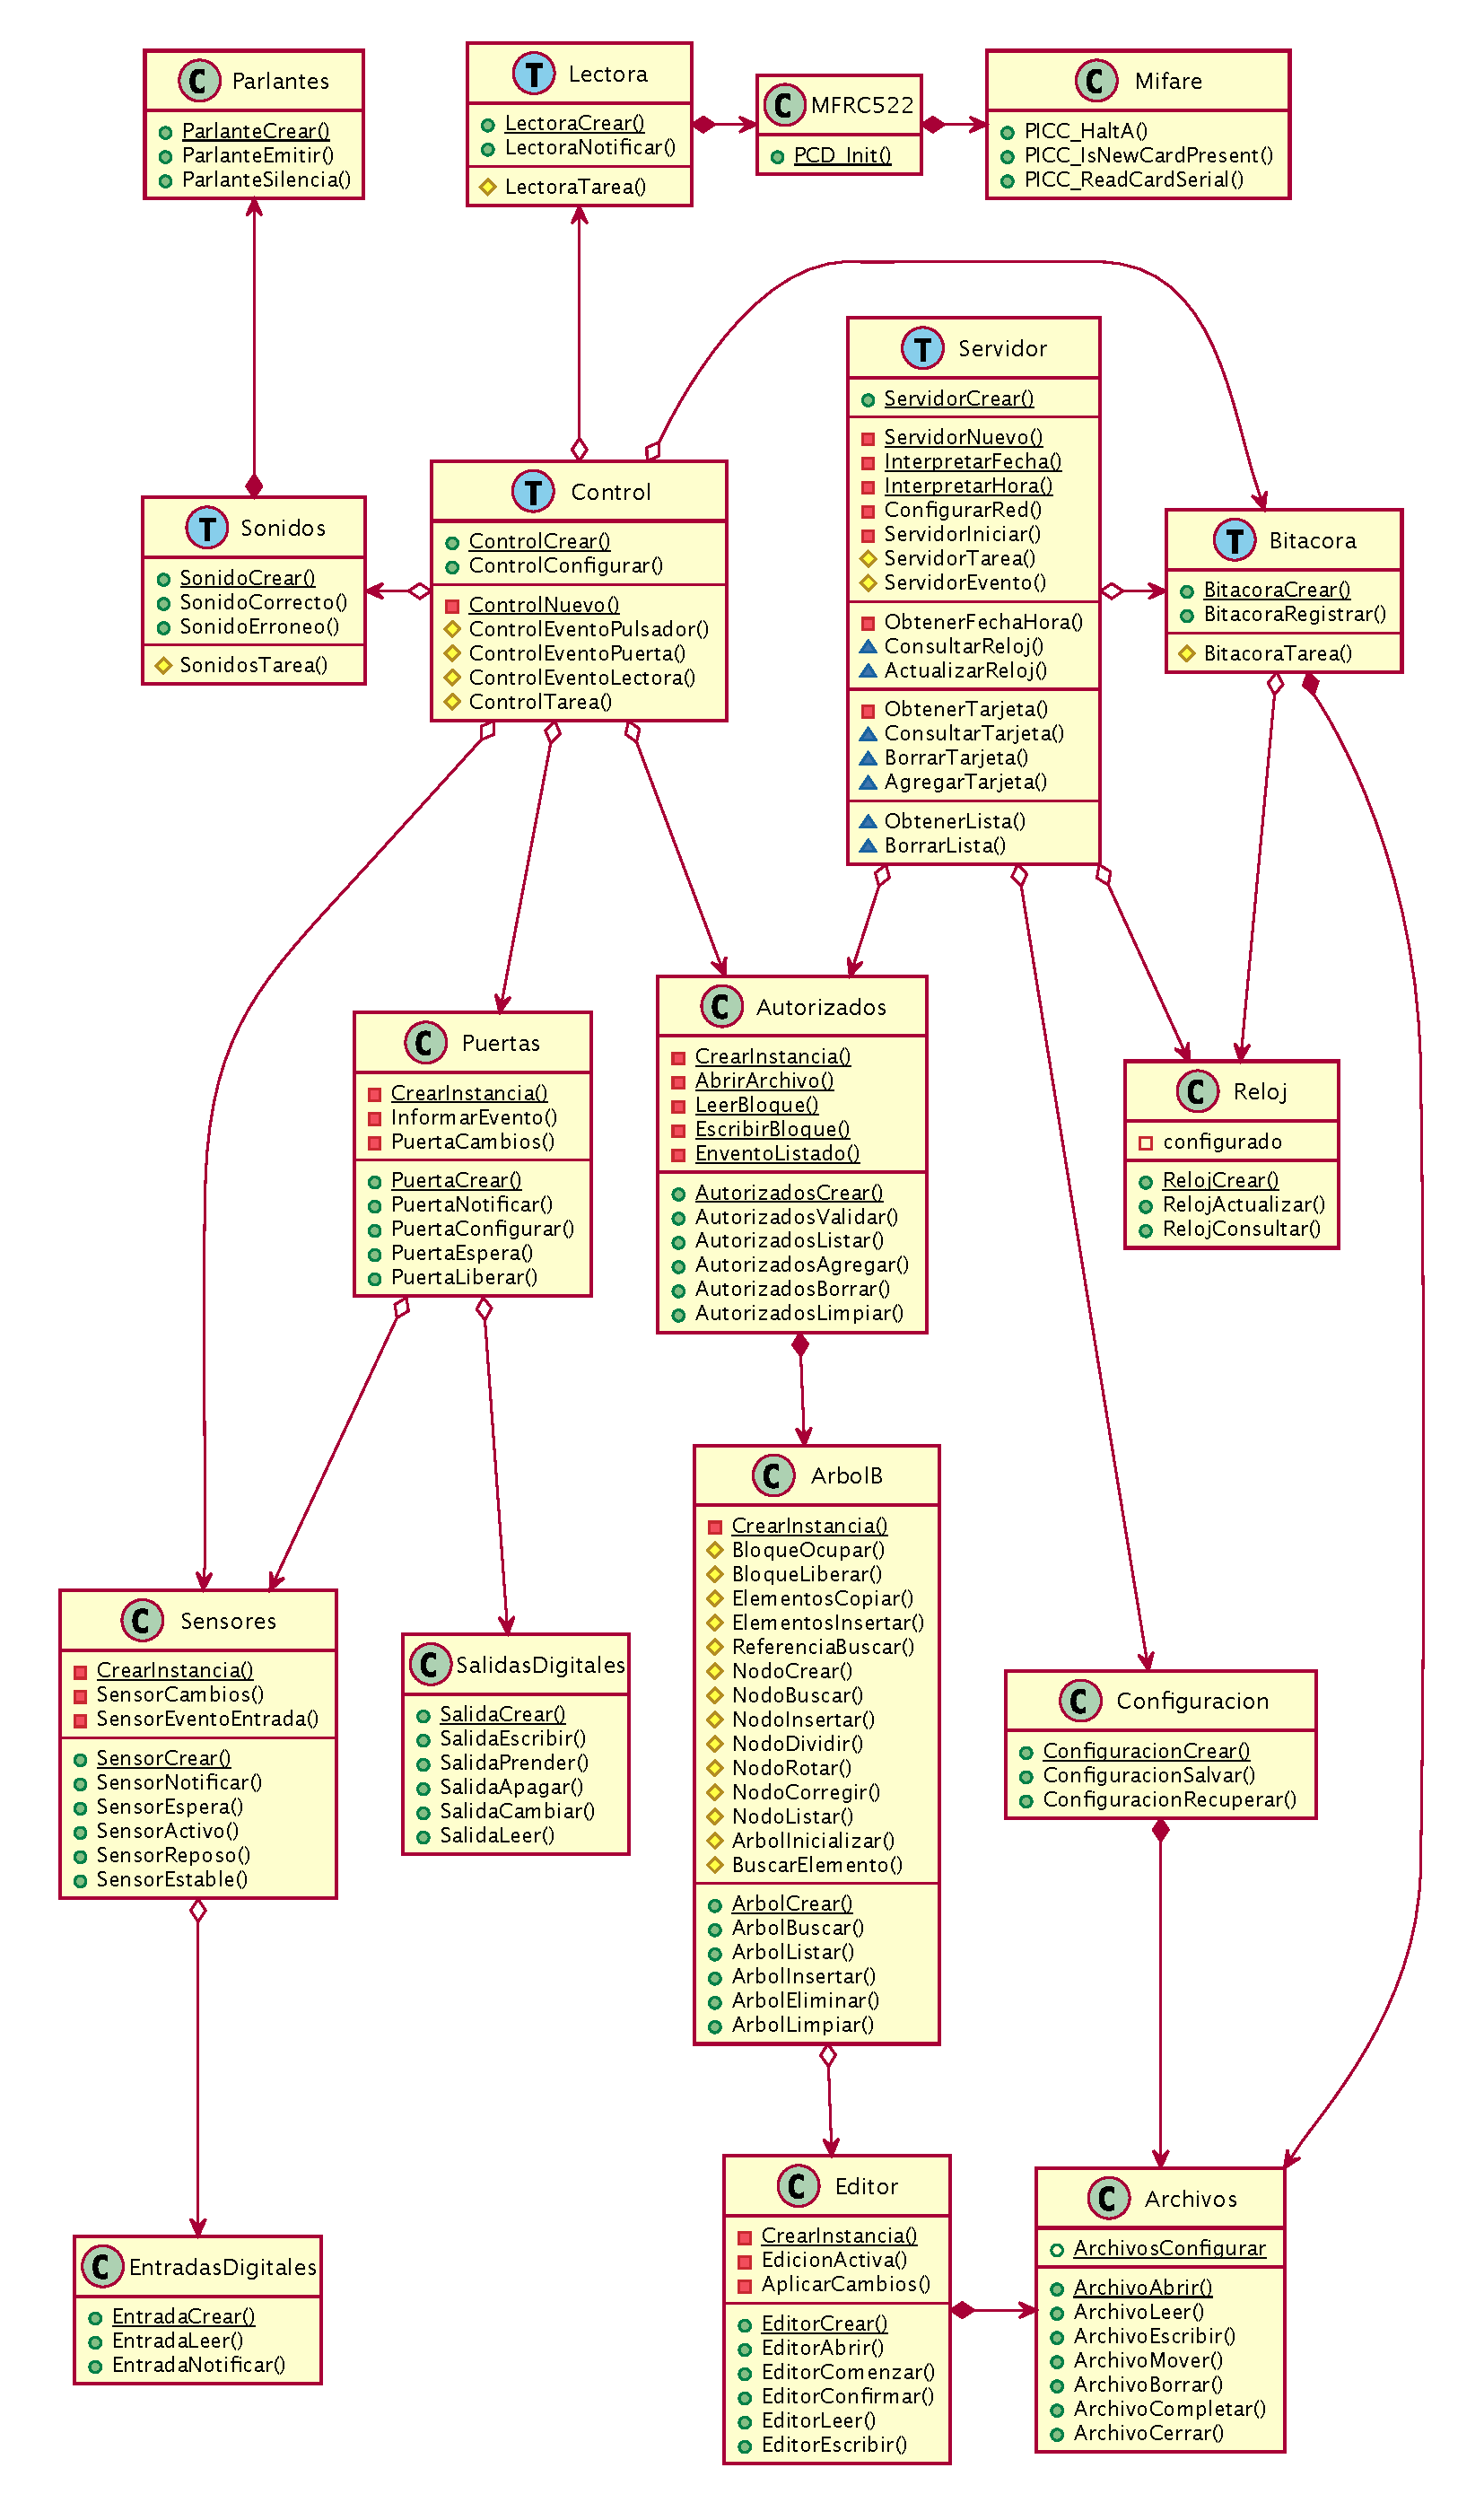
\includegraphics[width=\textwidth]{./Figures/PNK-DC002.pdf}
	\caption[Diagrama de clases del firmware del equipo]{Diagrama de clases del firmware del equipo.}
	\label{fig:DiagramaClases}
\end{figure}

\subsection{Capa de abstracción del hardware}

Esta capa contiene una colección de clases que encapsulan las funcionalidades del entorno de desarrollo provisto por el fabricante. Su principal objetivo es brindar una plataforma uniforme en comportamiento y documentación para el resto del firmware. Las clases que pertenecen a esta capa son:

\begin{itemize}
	\item EntradasDigitales: encapsula toda la gestión de un terminal digital utilizado como entrada. Permite configurarlo durante la creación del objeto, recuperar el estado actual y solicitar el envío de eventos generados por interrupciones disparadas por cambios en su estado.
	
	\item SalidasDigitales: encapsula toda la gestión de un terminal digital utilizado como salida. Permite configurarlo durante la creación del objeto, recuperar el estado actual y cambiarle el estado.
	
	\item Archivos: encapsula toda la gestión de un archivo almacenado en la tarjeta microSD del equipo. Después de la configuración de la propia clases permite la creación y el borrado de archivos, como así también la escritura y lectura de datos en ellos.
	
	\item Reloj: encapsula toda la gestión del reloj de tiempo real. Permite ajustar y recuperar la fecha y hora actuales.
	
	\item Parlantes: encapsula la gestión de un parlante conectado a un terminal digital que opera con modulación de ancho de pulso, o PWM (\emph{Pulse Width Modulation}). Permite, mediante la generación de una señal cuadrada de frecuencia arbitraria, emitir un tono en el parlante o silenciarlo.
\end{itemize}

\subsection{Capa de controladores}

Las clases que componen esta capa son independientes de la plataforma y de la aplicación, y por lo tanto son fácilmente reutilizables en otros proyectos. Para lograr este objetivo, la mayoría de ellas no utilizan  los servicios del sistema operativo, e implementan mecanismos de eventos para  extraer el código dependiente de la aplicación en otro componente. Las clases que pertenecen a esta capa son:

\begin{itemize}
	\item Puertas: encapsula toda la gestión de la puerta. Permite configurar el tipo de cerradura, habilitar o ignorar el sensor de puerta abierta y definir los tiempos correspondientes de liberación, apertura y cierre. Puede generar eventos cuando se completa un ciclo de apertura. Esta clase tiene una especial importancia en el sistema, ya que la misma implementa aproximadamente el 30\% de los requisitos funcionales definidos en la sección \ref{sec:Requisitos}. Para la implementación se optó por utilizar cuatro maquinas de estado finitos independientes, una para cada modo de funcionamiento descrito en la tabla \ref{tab:ModosOperacion}. Para modelar las mismas se utilizaron diagramas de estado UML, los cuales se pueden ver en las figuras \ref{fig:ControlSinSin}, \ref{fig:ControlSinCon}, \ref{fig:ControlConSin} y \ref{fig:ControlConCon}

\begin{figure}[H]
	\centering
	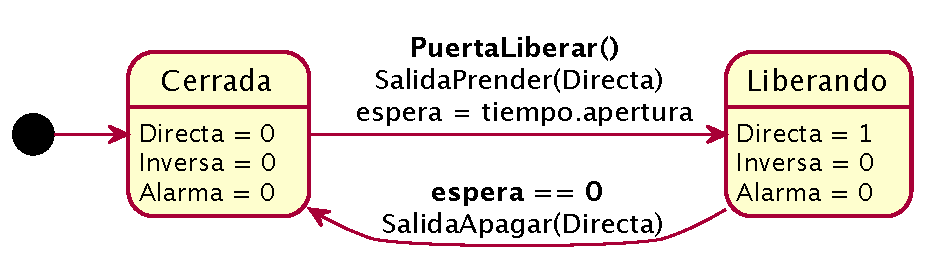
\includegraphics[width=0.9\textwidth]{Figures/PNK-DE001.pdf}
	\caption[Diagrama de estados con cerradura electromagnética y sin sensor]{Diagrama de estado para el control de una puerta sin sensor de apertura y con liberación electromagnética.}
	\label{fig:ControlSinSin}
\end{figure}

\begin{figure}[H]
	\centering
	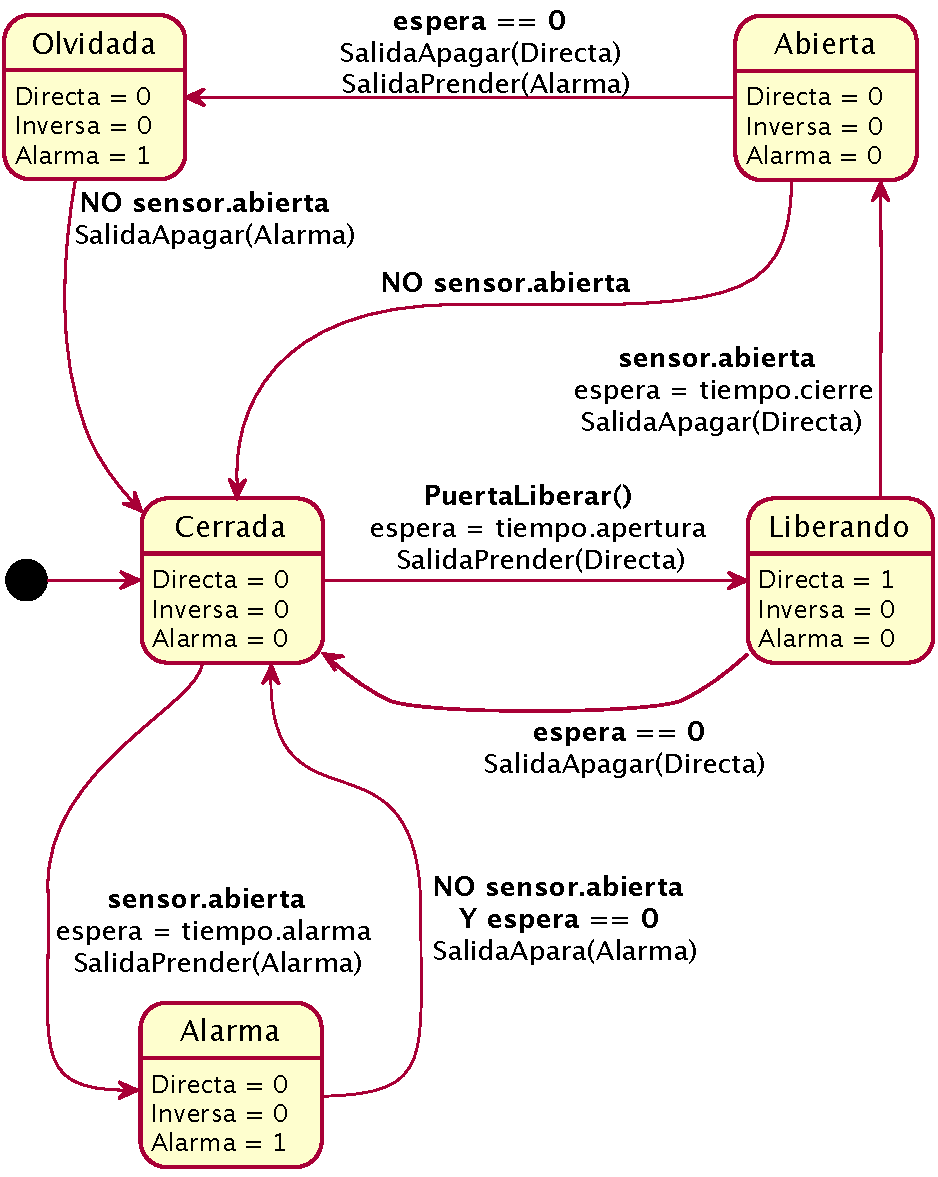
\includegraphics[width=0.9\textwidth]{Figures/PNK-DE002.pdf}
	\caption[Diagrama de estados con cerradura electromagnética y sensor]{Diagrama de estado para el control de una puerta con sensor de apertura y con liberación electromagnética.}
	\label{fig:ControlSinCon}
\end{figure}

\begin{figure}[H]
	\centering
	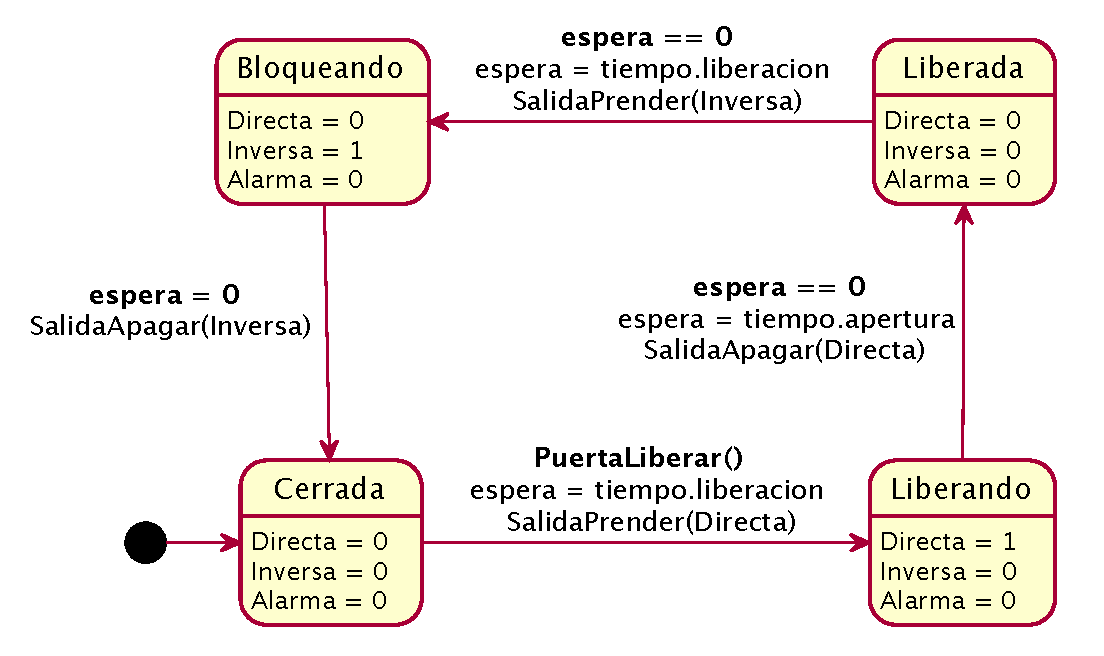
\includegraphics[width=0.9\textwidth]{Figures/PNK-DE003.pdf}
	
	\caption[Diagrama de estados con cerradura motorizada y sin sensor]{Diagrama de estado para el control de una puerta sin sensor de apertura y con liberación motorizada.}
	\label{fig:ControlConSin}
\end{figure}

\begin{figure}[ht]
	\centering
	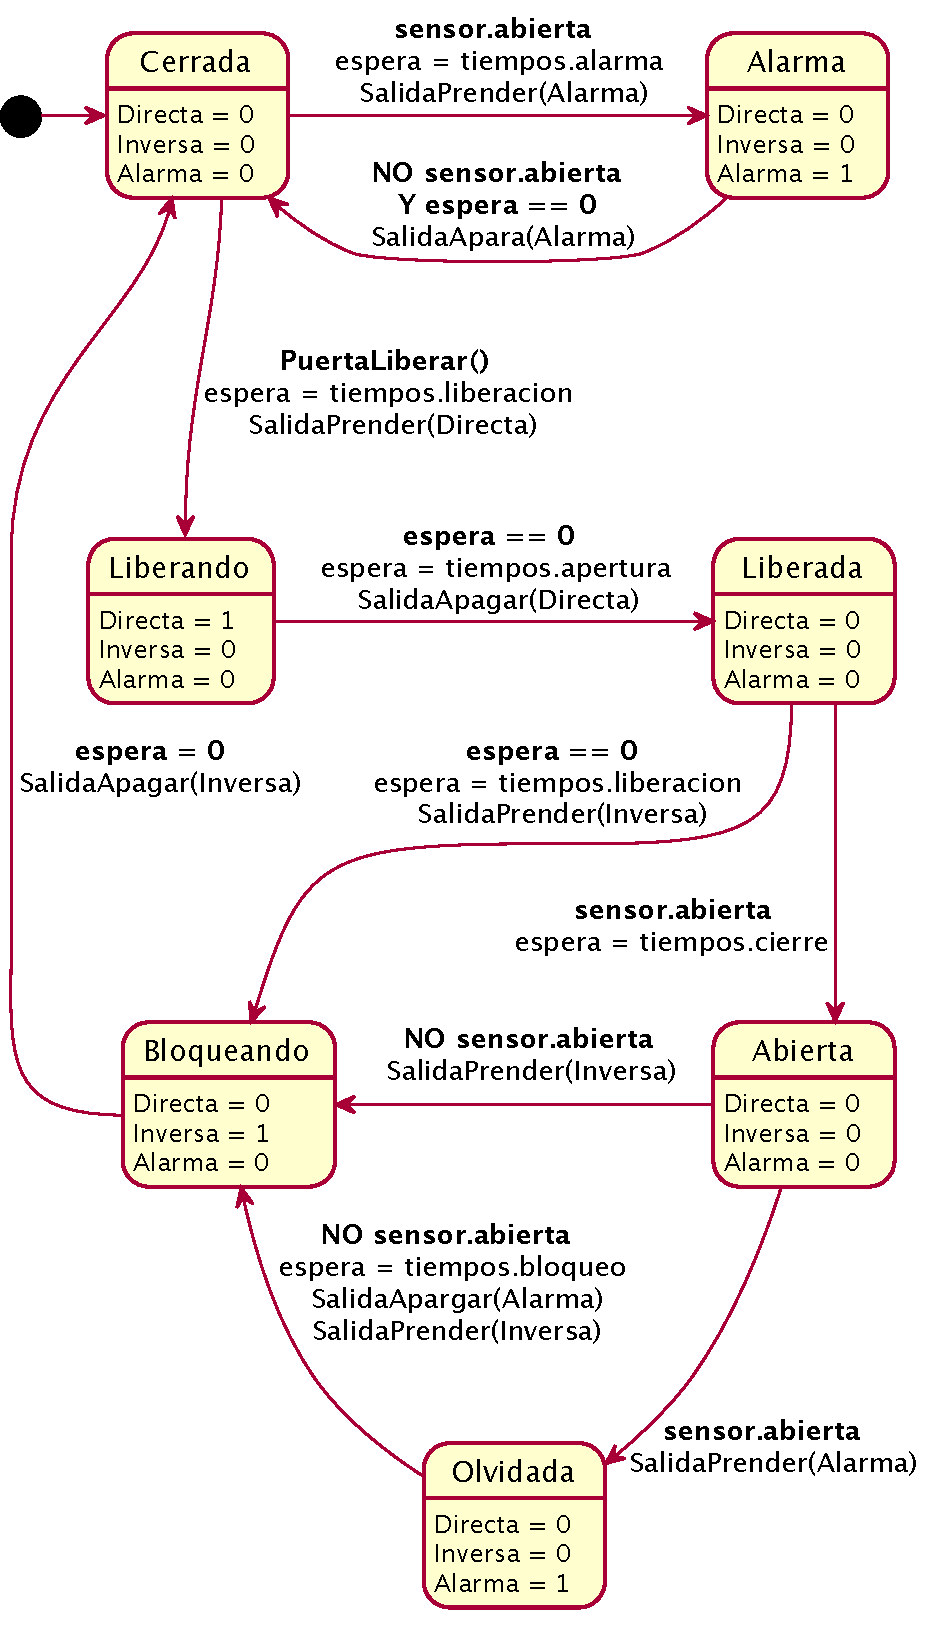
\includegraphics[width=0.9\textwidth]{Figures/PNK-DE004.pdf}
	\caption[Diagrama de estados con cerradura motorizada y sensor]{Diagrama de estado para el control de una puerta con sensor de apertura y con liberación motorizada.}
	\label{fig:ControlConCon}
\end{figure}
	
	\item ArbolB: encapsula toda la gestión de un índice utilizando la estructura de datos denominada ArbolB  o \emph{BTree}. Permite aprovechar las transferencias de bloques en los almacenamientos secundarios, como la tarjeta microSD, para disminuir el tiempo de búsqueda y actualización de una lista ordenada. Tanto la clase Editor, que se explica a continuación, como esta son también componentes críticos del sistema, ya que cualquier error en ellas se traduce en que personas autorizadas no puedan ingresar, o peor aún, en accesos de personas no autorizadas. Pero a diferencia de la clase Puertas, en estas el aspecto crítico está en la implementación y no en el diseño, ya que los algoritmos que se utilizan son ampliamente conocidos.
		
	\item Editor: encapsula toda la gestión de una actualización que involucra múltiples escrituras en un archivo. Permite asegurar que el contenido del índice de tarjetas autorizadas no resultará corrupto por una modificación incompleta. Esta clase utiliza el concepto de transacción ACID (\emph{Atomicity, Consistency, Isolation and Durability)} muy común en las bases de datos relacionales, que en nuestro caso se puede resumir en que cualquier cambio al índice se realiza siempre de manera completa, o de lo contrario, no efectúa absolutamente ningún cambio. Para la implementación se utilizó un archivo de transacciones donde se registran las escrituras de los sectores que se van actualizando en el índice. Al completar la modificación, esta se confirma en el mismo archivo de transacciones, y a partir de este punto se comienzan a aplicar los cambios en el archivo de datos. Si ocurre una interrupción del proceso, por ejemplo por un reinicio del sistema, primero se buscan transacciones confirmadas para aplicar los cambios nuevamente y recién entonces se comienza la operación del sistema.

\FloatBarrier

	\item Autorizados: encapsula toda la gestión de una lista con las tarjetas autorizadas a ingresar. Permite consultar si una tarjeta está autorizada, recuperar toda la lista de tarjetas autorizadas y agregar o eliminar una tarjeta en ella. Esta clase agrega muy poca lógica y es prácticamente un adaptador de la clase ArbolB para convertir la funcionalidad de un índice en una lista presente/ausente. Esta clase agrega además el control de sección crítica necesario para que el índice pueda ser consultado y actualizado por dos tareas diferentes que se ejecutan en forma concurrente.

	\item Sensores: encapsula toda la gestión de filtro digital asociado a terminales digitales de entrada. Permite definir un valor de histéresis para eliminar los eventos generados por ruido electromagnético. También permite generar eventos por cambios en el estado del sensor y determinar si la entrada digital presenta un estado estable o se encuentra en transición.

	\item Configuración: encapsula toda la gestión de las opciones de configuración del equipo. Permite consolidar las opciones que pueden cambiar en cada uno de los componentes en una estructura binaria, que puede ser convertida desde y hacia una cadena de caracteres utilizando la codificación JSON.
\end{itemize}


\subsection{Tareas del sistema}

En esta capa se encuentran las clases que implementan directamente la lógica de funcionamiento del equipo con el  mayor nivel de abstracción. Esto permite extender la funcionalidad en forma simple, dado que el código aplica, casi directamente, las reglas de negocio del equipo. Todas las clases de esta capa encapsulan tareas del sistema operativo de tiempo real que se ejecutan en forma concurrente. Las clases que componen esta capa son:

\begin{itemize}
	\item Sonidos: encapsula toda la reproducción de una melodía monofónica en un parlante. Define una secuencia de notas especificando la frecuencia y duración de las mismas, y de esta manera permite generar dos sonidos distintivos para diferenciar los accesos autorizados de los rechazados.
	
	\item Lectora: encapsula toda la comunicación con la lectora y, por medio de esta, con la tarjeta de proximidad. Permite recuperar el número de serie único asignado a la tarjeta y genera un evento al control para informar de una nueva lectura.

	\item Control: encapsula toda la gestión de las reglas para la apertura y supervisión de la puerta. Esta clase implementa un patrón de diseño de software denominado control ambiental. De esta forma convergen en un solo punto los eventos de la clase Puerta, de la clase Sensor, de la clase Lectora y de la clase Autorizados para centralizar la respuesta y el registro a estos eventos. 
	
	\item Bitacora: encapsula el proceso de registro en un archivo de los eventos generados por el control. Permite efectuar la escritura en el archivo, una operación lenta, en forma diferida para minimizar la interferencia en los tiempos de operación del control de la puerta.
	
	\item Servidor: encapsula todo el servicio de comunicación para la gestión del equipo. Permite configurar la interfaz WiFi, iniciar un servidor HTTP y atender los pedidos recibidos interactuando con las clases Reloj, Bitacora, Configuracion y Autorizados para completar las operaciones solicitadas.
	
\end{itemize}

De la descripción anterior se desprende que la correcta interacción entre las clases de esta capa resulta clave para lograr el funcionamiento esperado del equipo. La ingeniería de software nos brinda una herramienta para poder representar estas interacciones entre los componentes de un programa: los diagramas de secuencia UML. En estos se representan las llamadas a métodos de las diferentes clases siguiendo los casos de uso analizados en la subsección \ref{sub:CasosDeUso}. Los diagramas más importantes pueden verse en las figuras \ref{fig:SecuanciaPulsador}, \ref{fig:SecuenciaTarjeta}, \ref{fig:SecuenciaForzada} y \ref{fig:SecuenciaConfiguracion}.

\begin{figure}[ht]
	\centering
	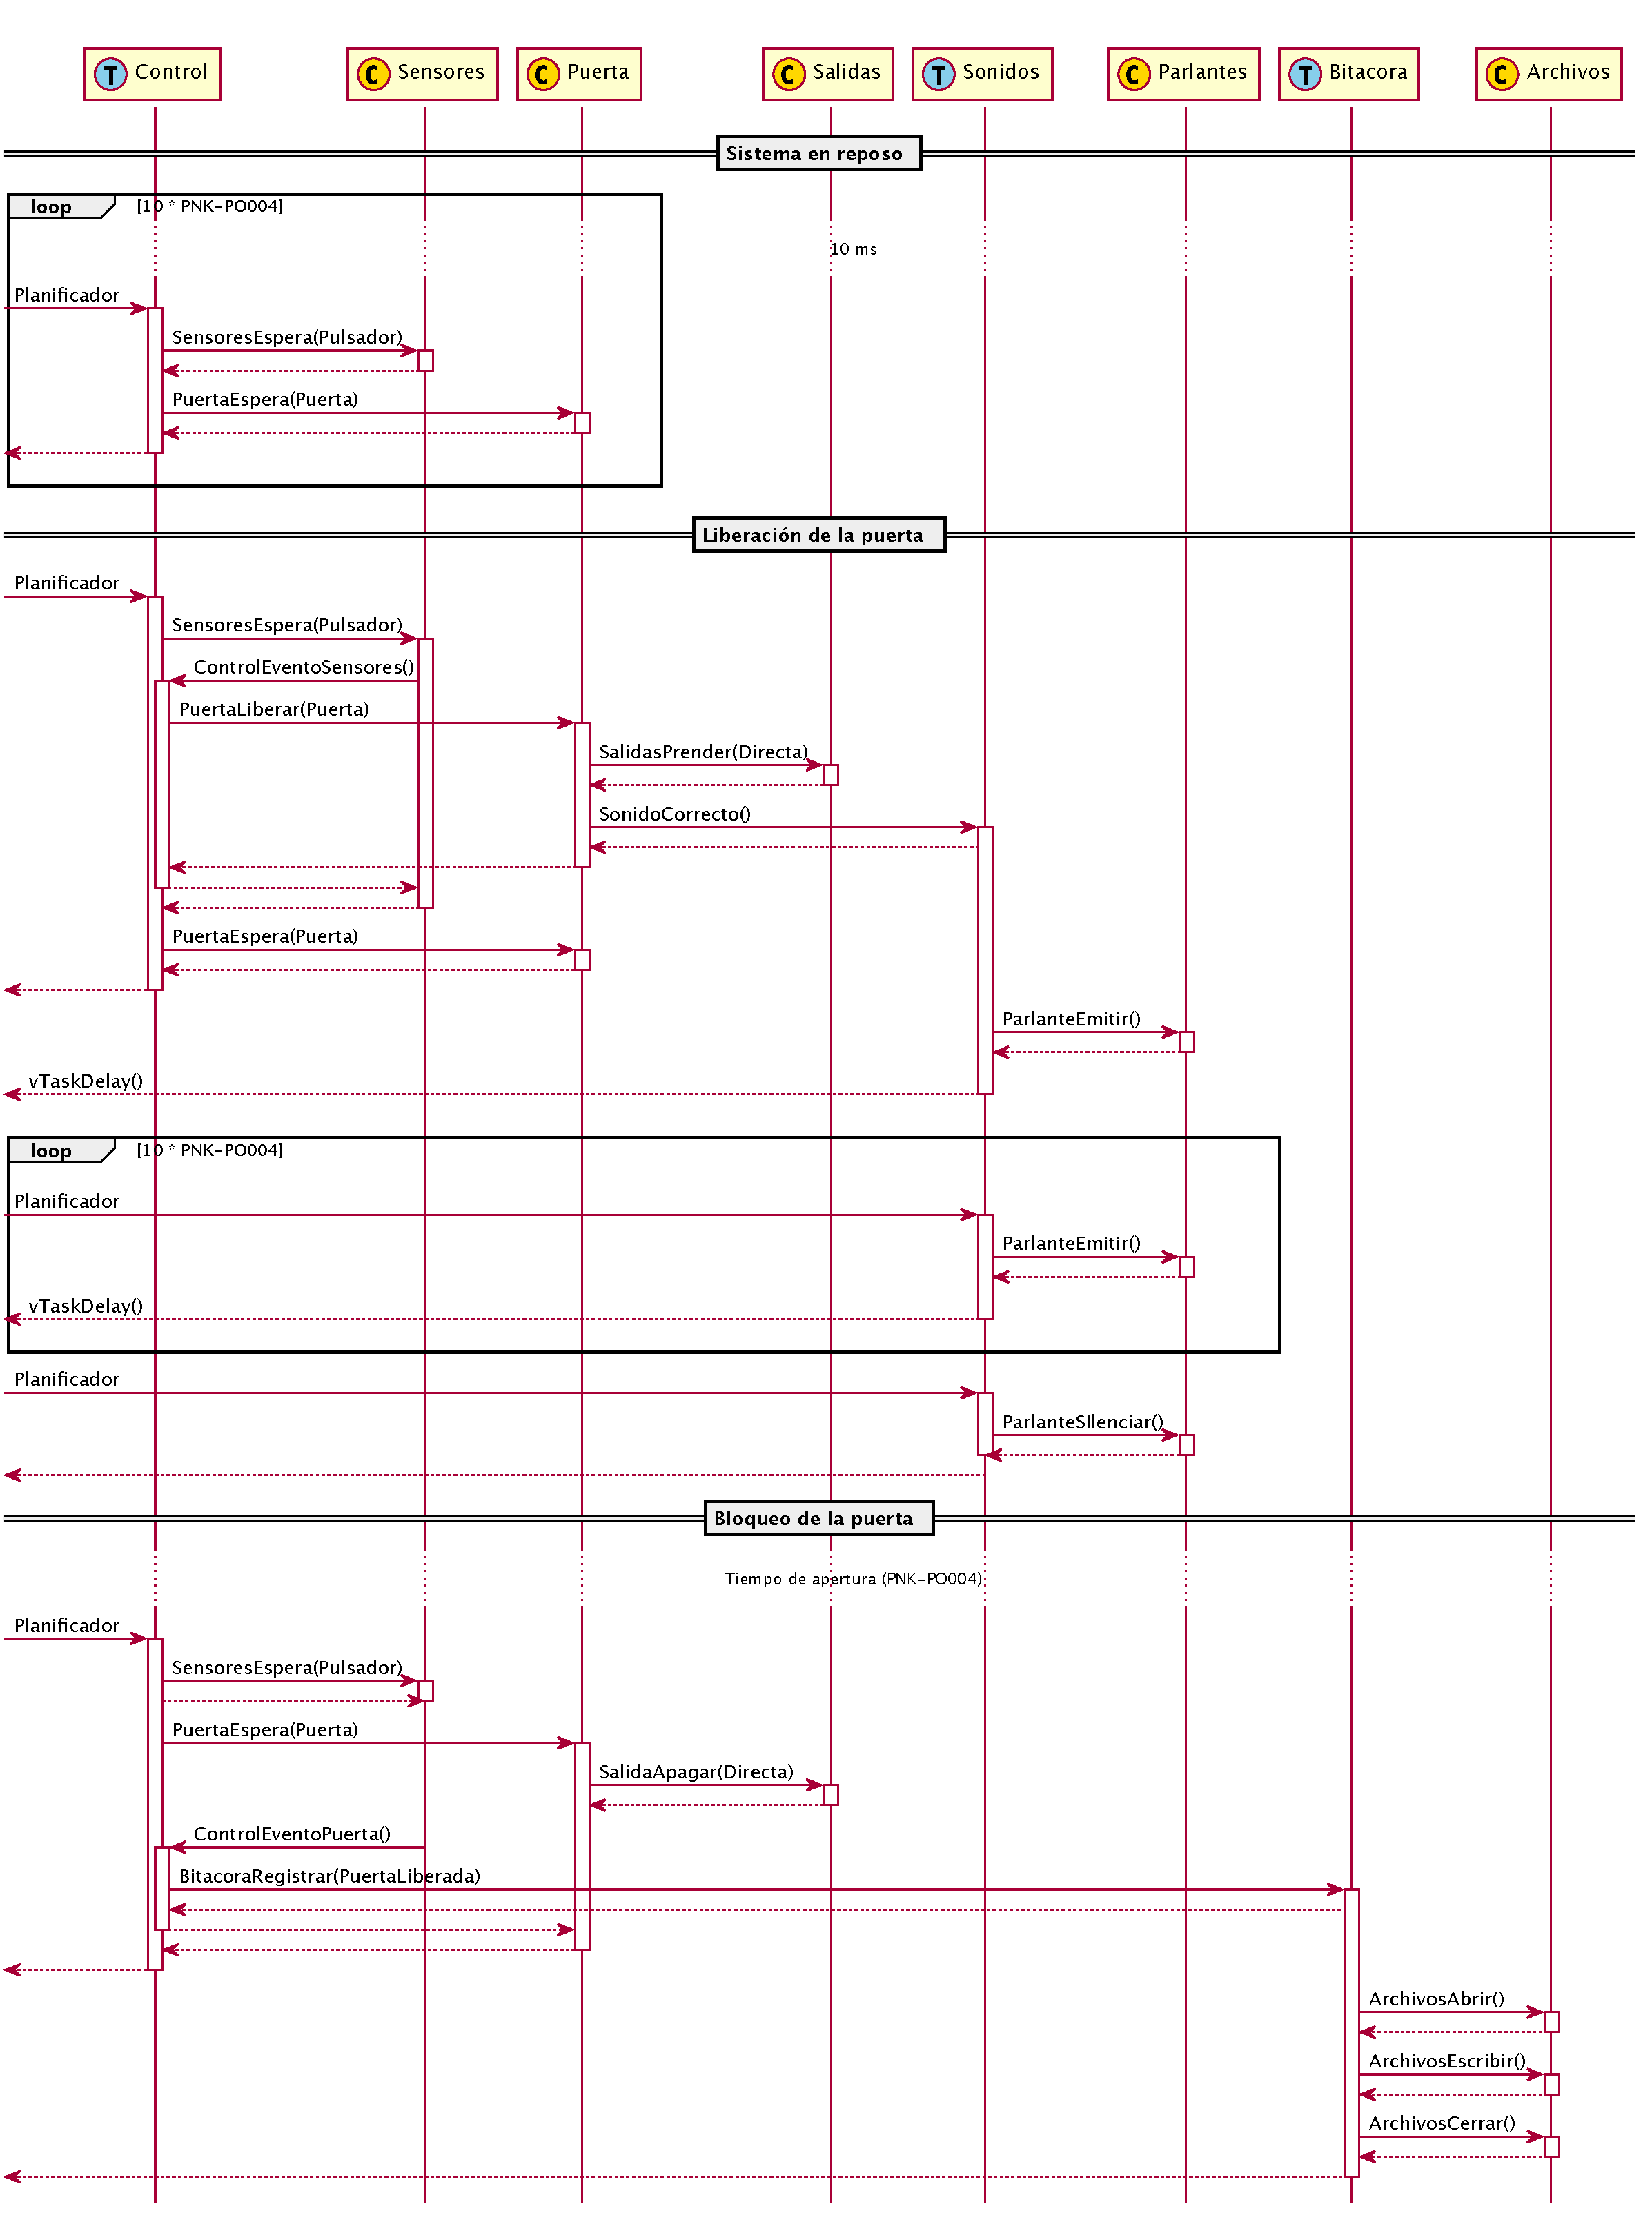
\includegraphics[width=\textwidth]{Figures/PNK-DS001.pdf}
	\caption[Apertura por pulsador con cerradura electromagnética y sin sensor]{Diagrama de secuencia para la liberación por pulsador de una puerta, sin sensor de apertura y con liberación electromagnética.}
	\label{fig:SecuanciaPulsador}
\end{figure}

\begin{figure}[ht]
	\centering
	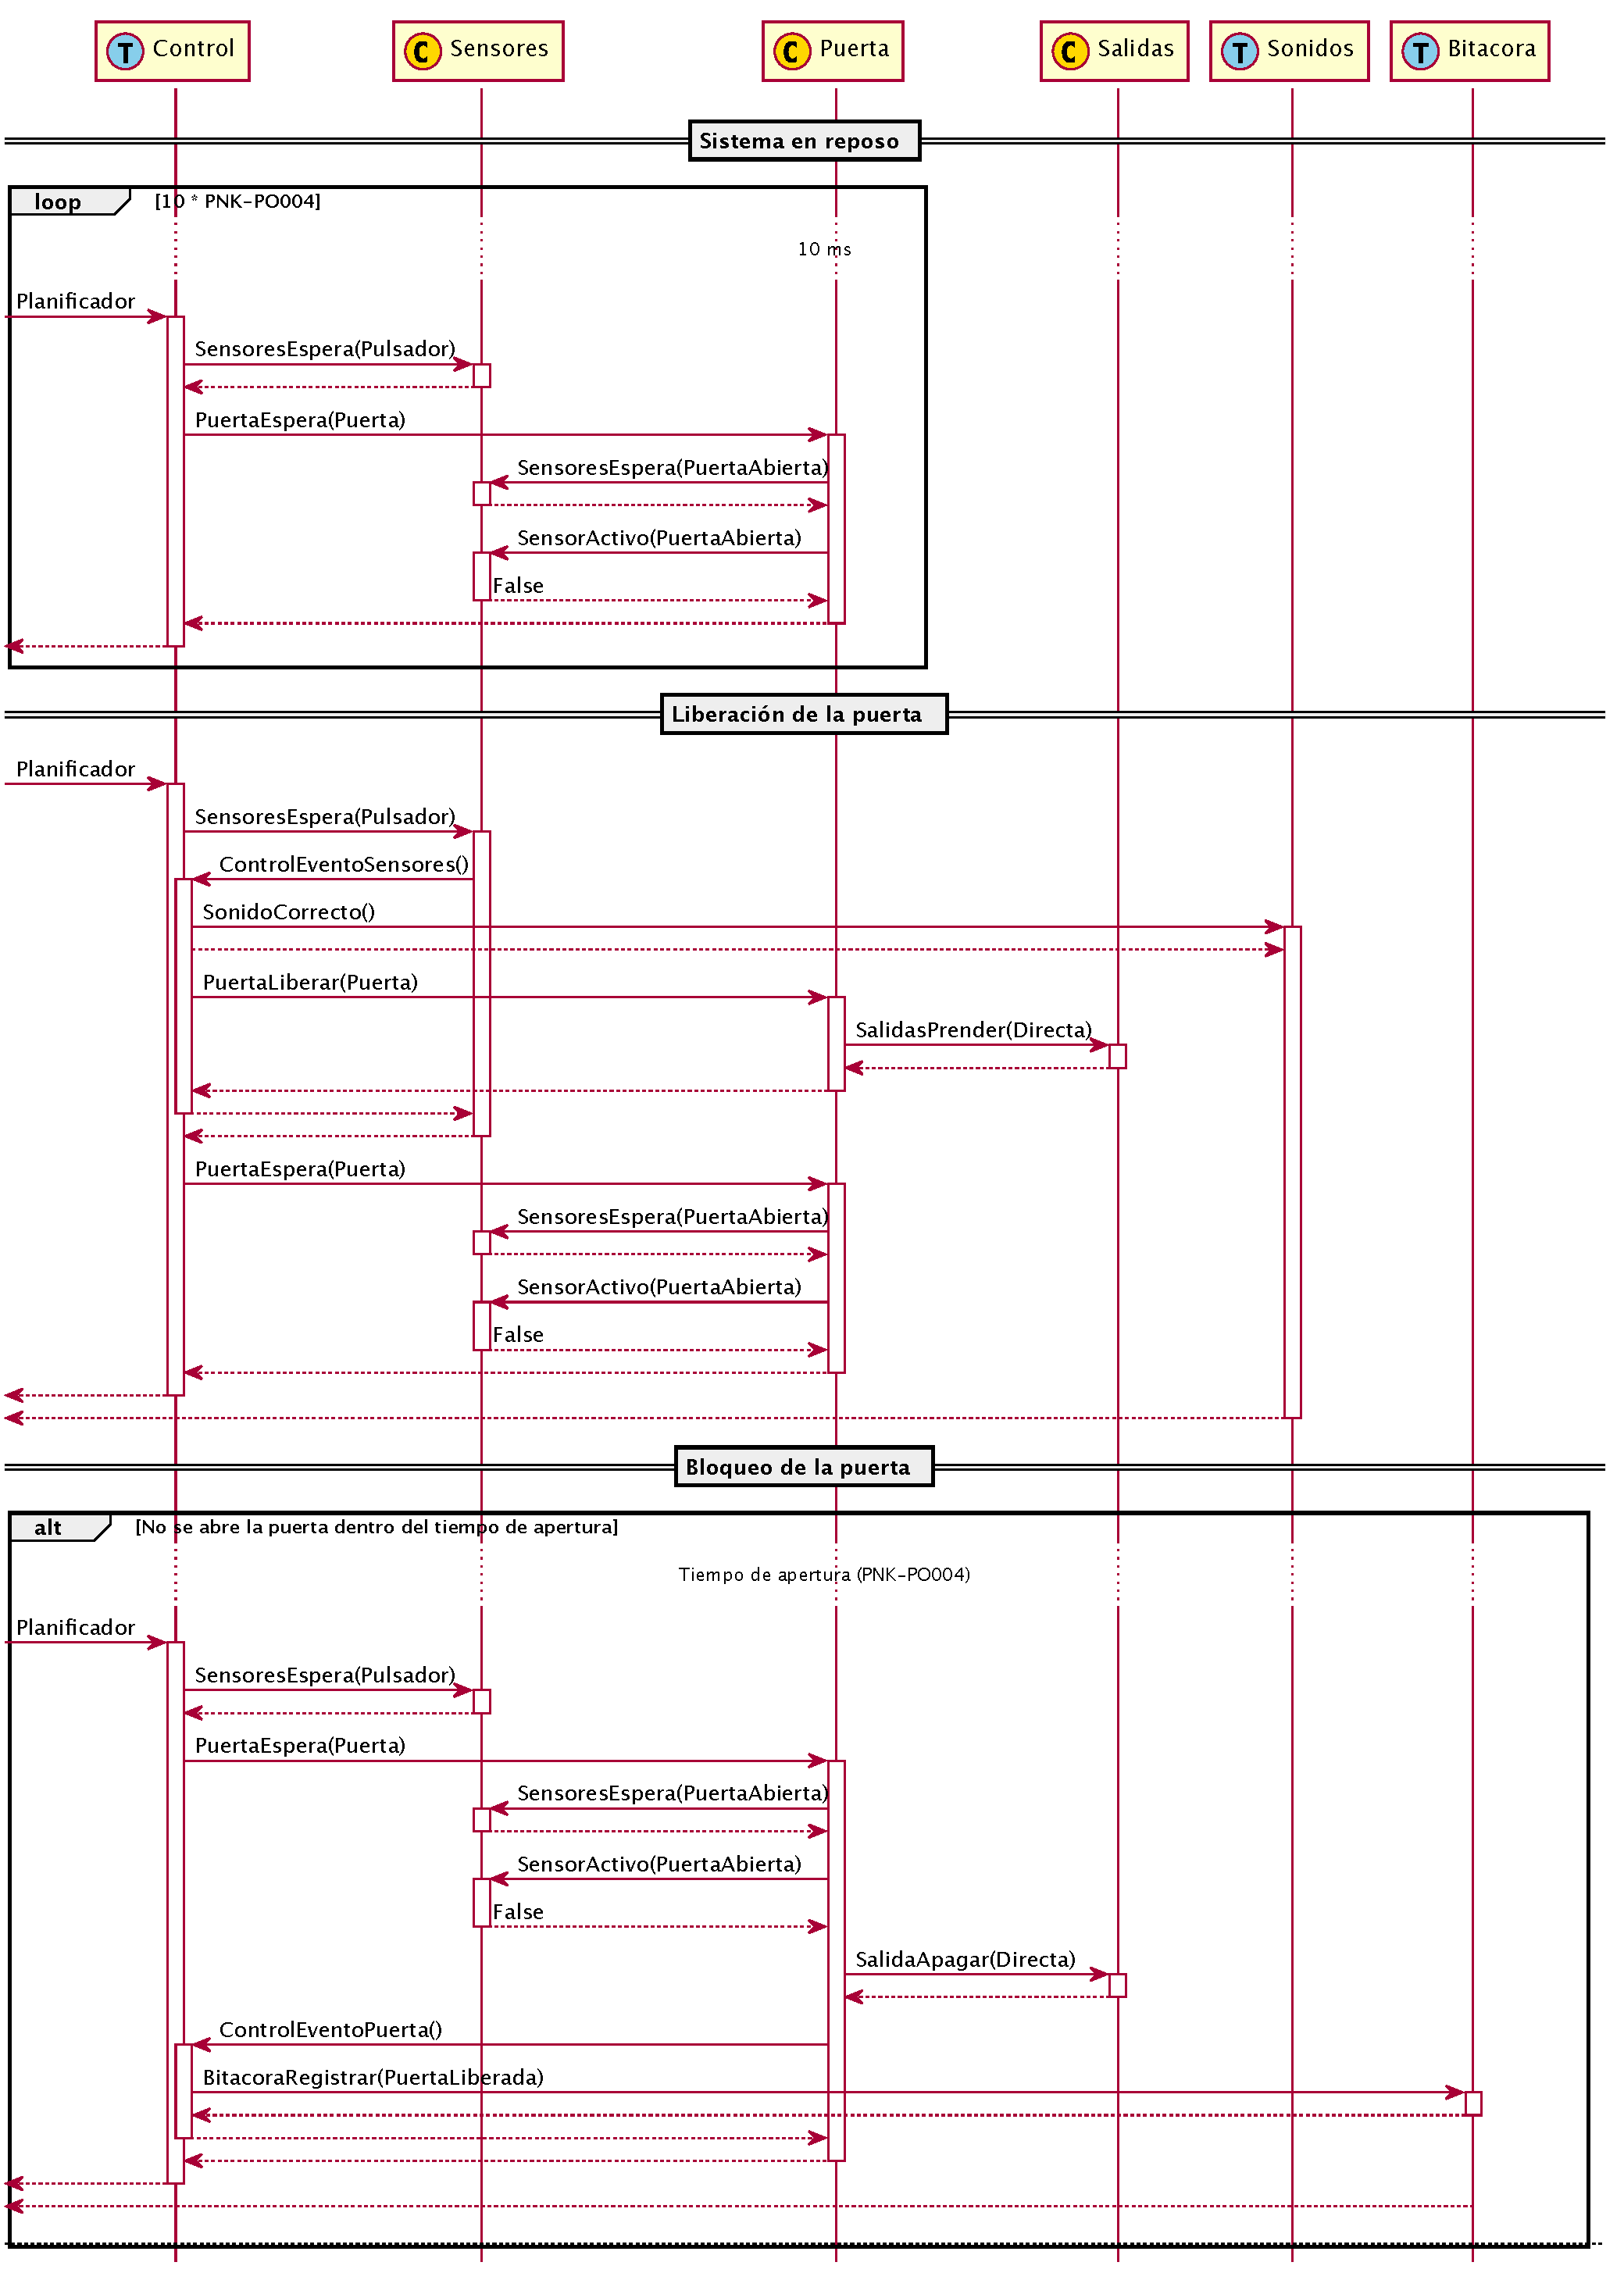
\includegraphics[width=\textwidth]{Figures/PNK-DS002-A.pdf}
	{\color{red} No es el diagrama correcto pero tiene la misma forma y extensión}
	\caption[Apertura por tarjeta con cerradura electromagnética y sensor]{Diagrama de secuencia para la apertura y cierre por tarjeta de proximidad, con sensor de apertura y con liberación electromagnética.}
	\label{fig:SecuenciaTarjeta}
\end{figure}

\begin{figure}[ht]
	\centering
	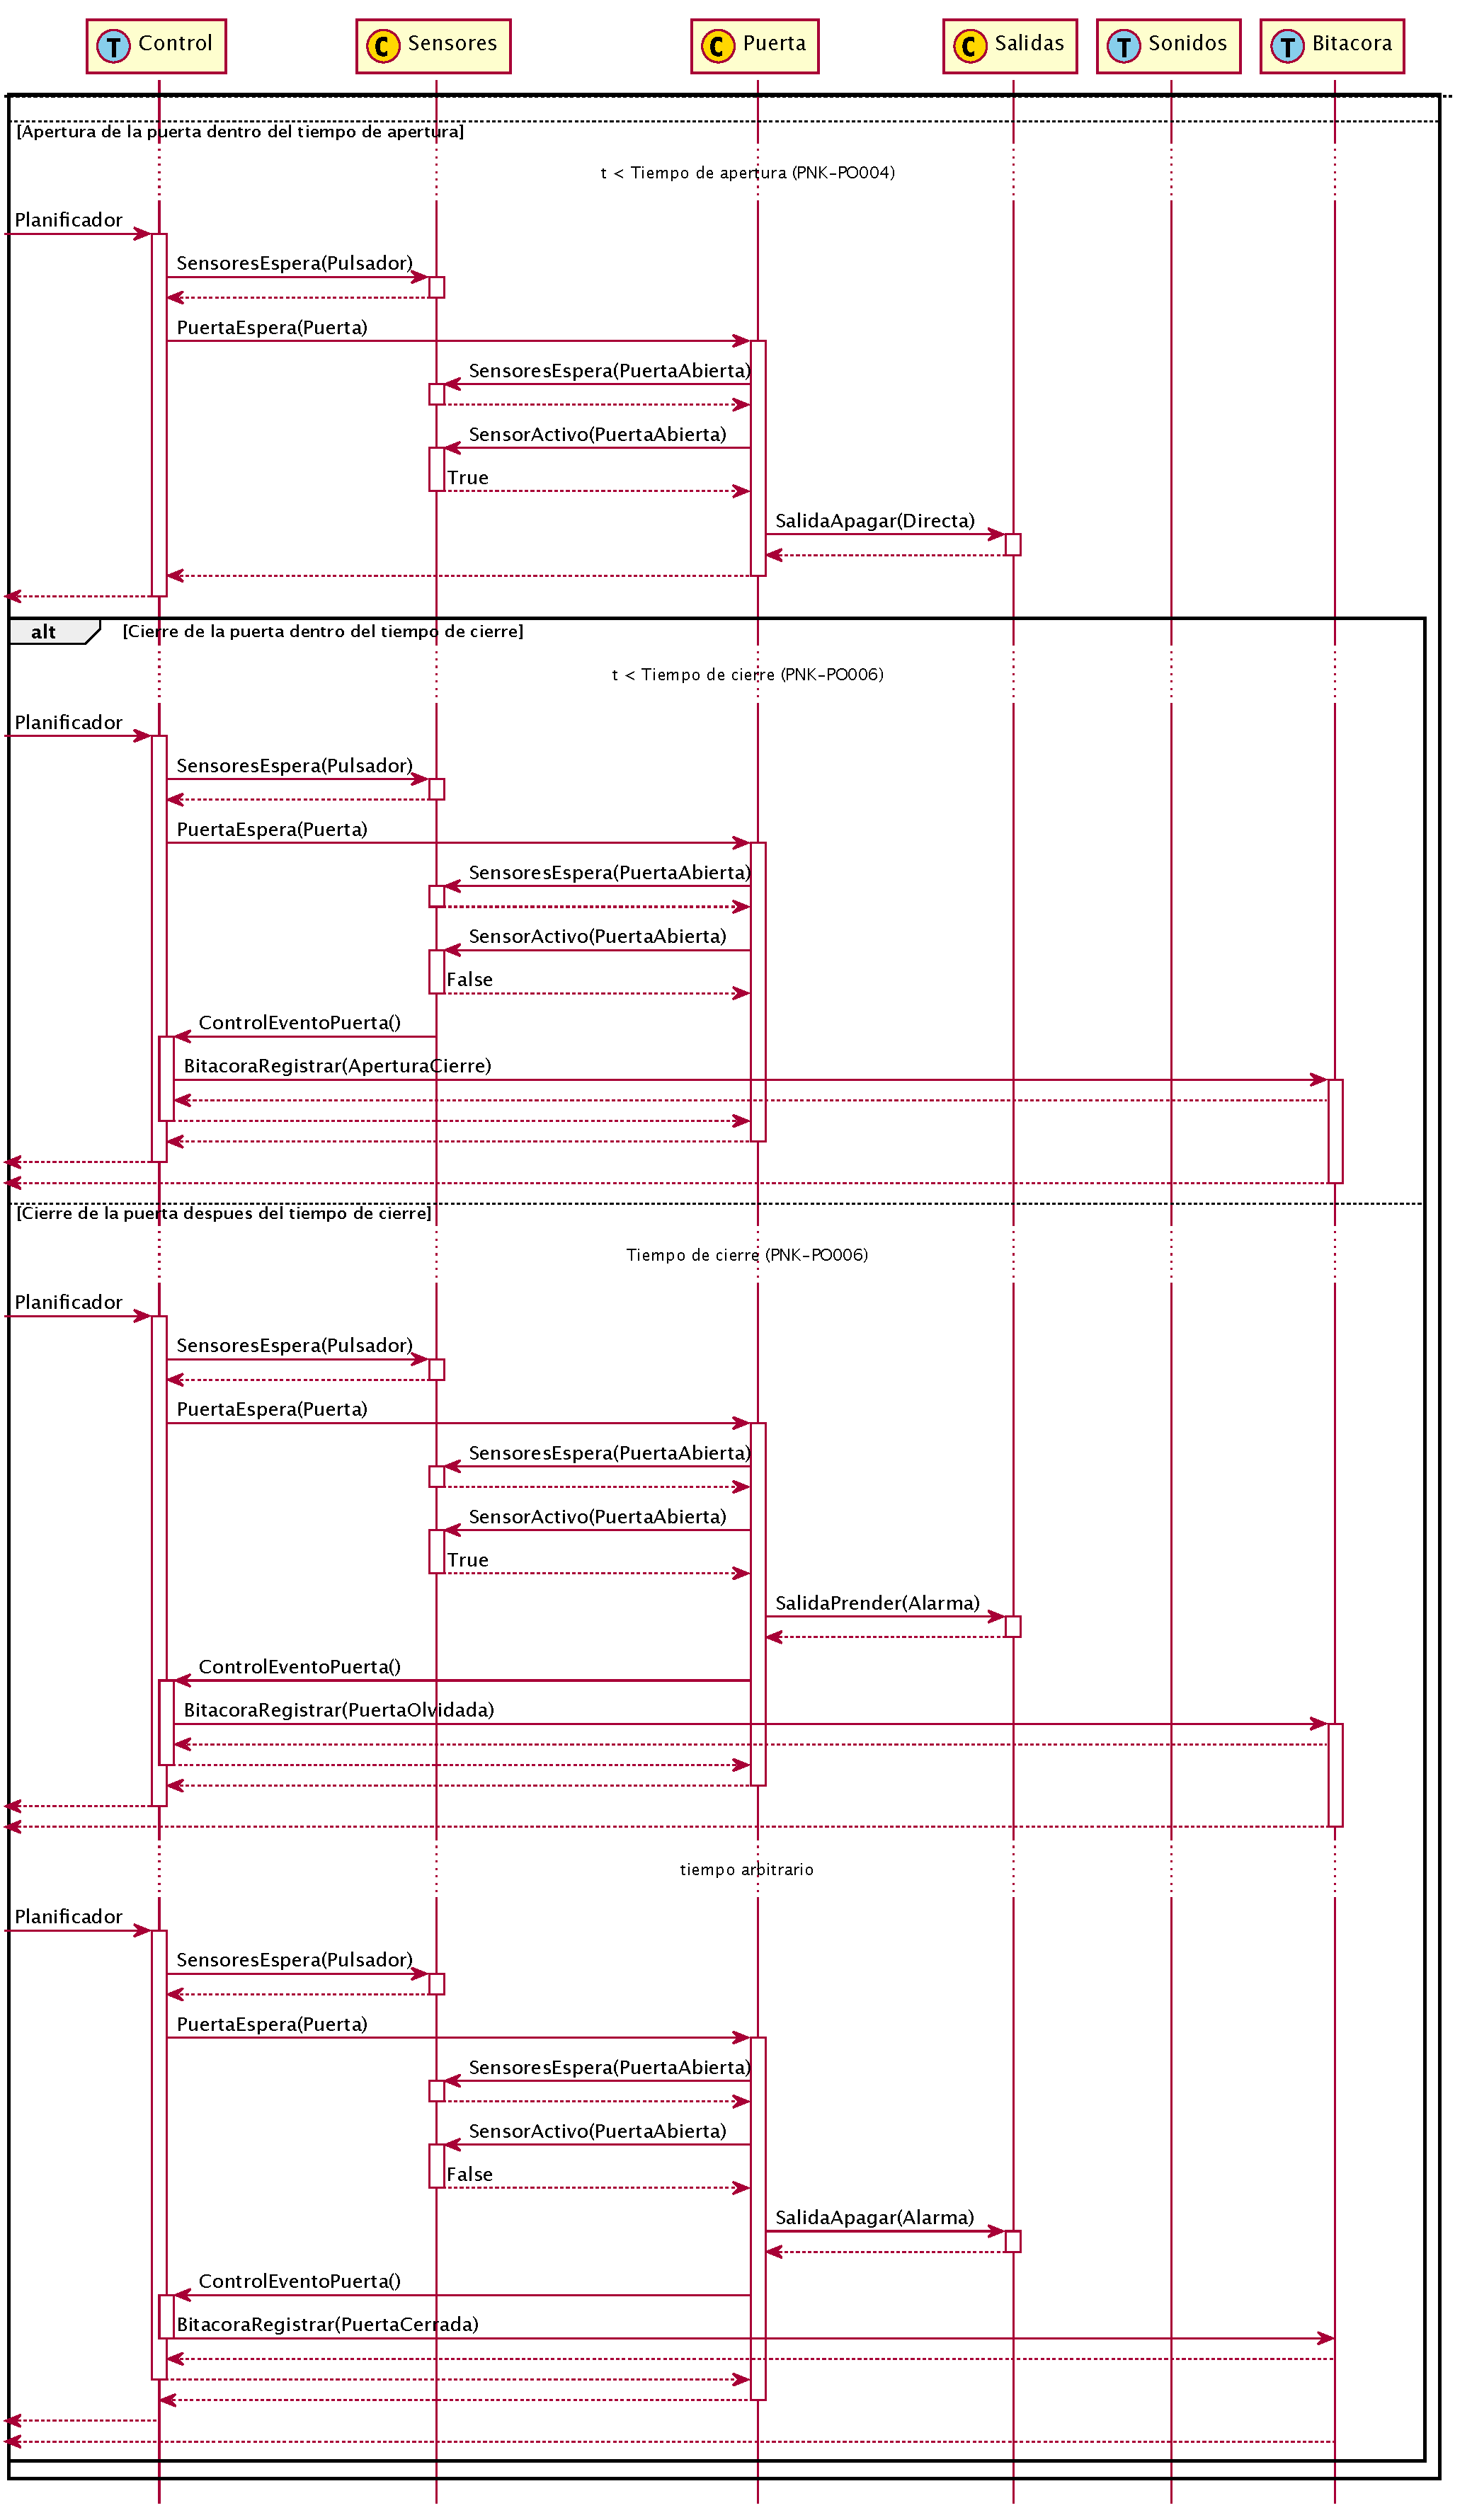
\includegraphics[width=\textwidth]{Figures/PNK-DS002-B.pdf}
	{\color{red} No es el diagrama correcto pero tiene la misma forma y extensión}
	\caption[Alarma por apertura forzada de la puerta]{Diagrama de secuencia para la activación de alarma por apertura forzada de la puerta.}
	\label{fig:SecuenciaForzada}
\end{figure}

\begin{figure}[ht]
	\centering
	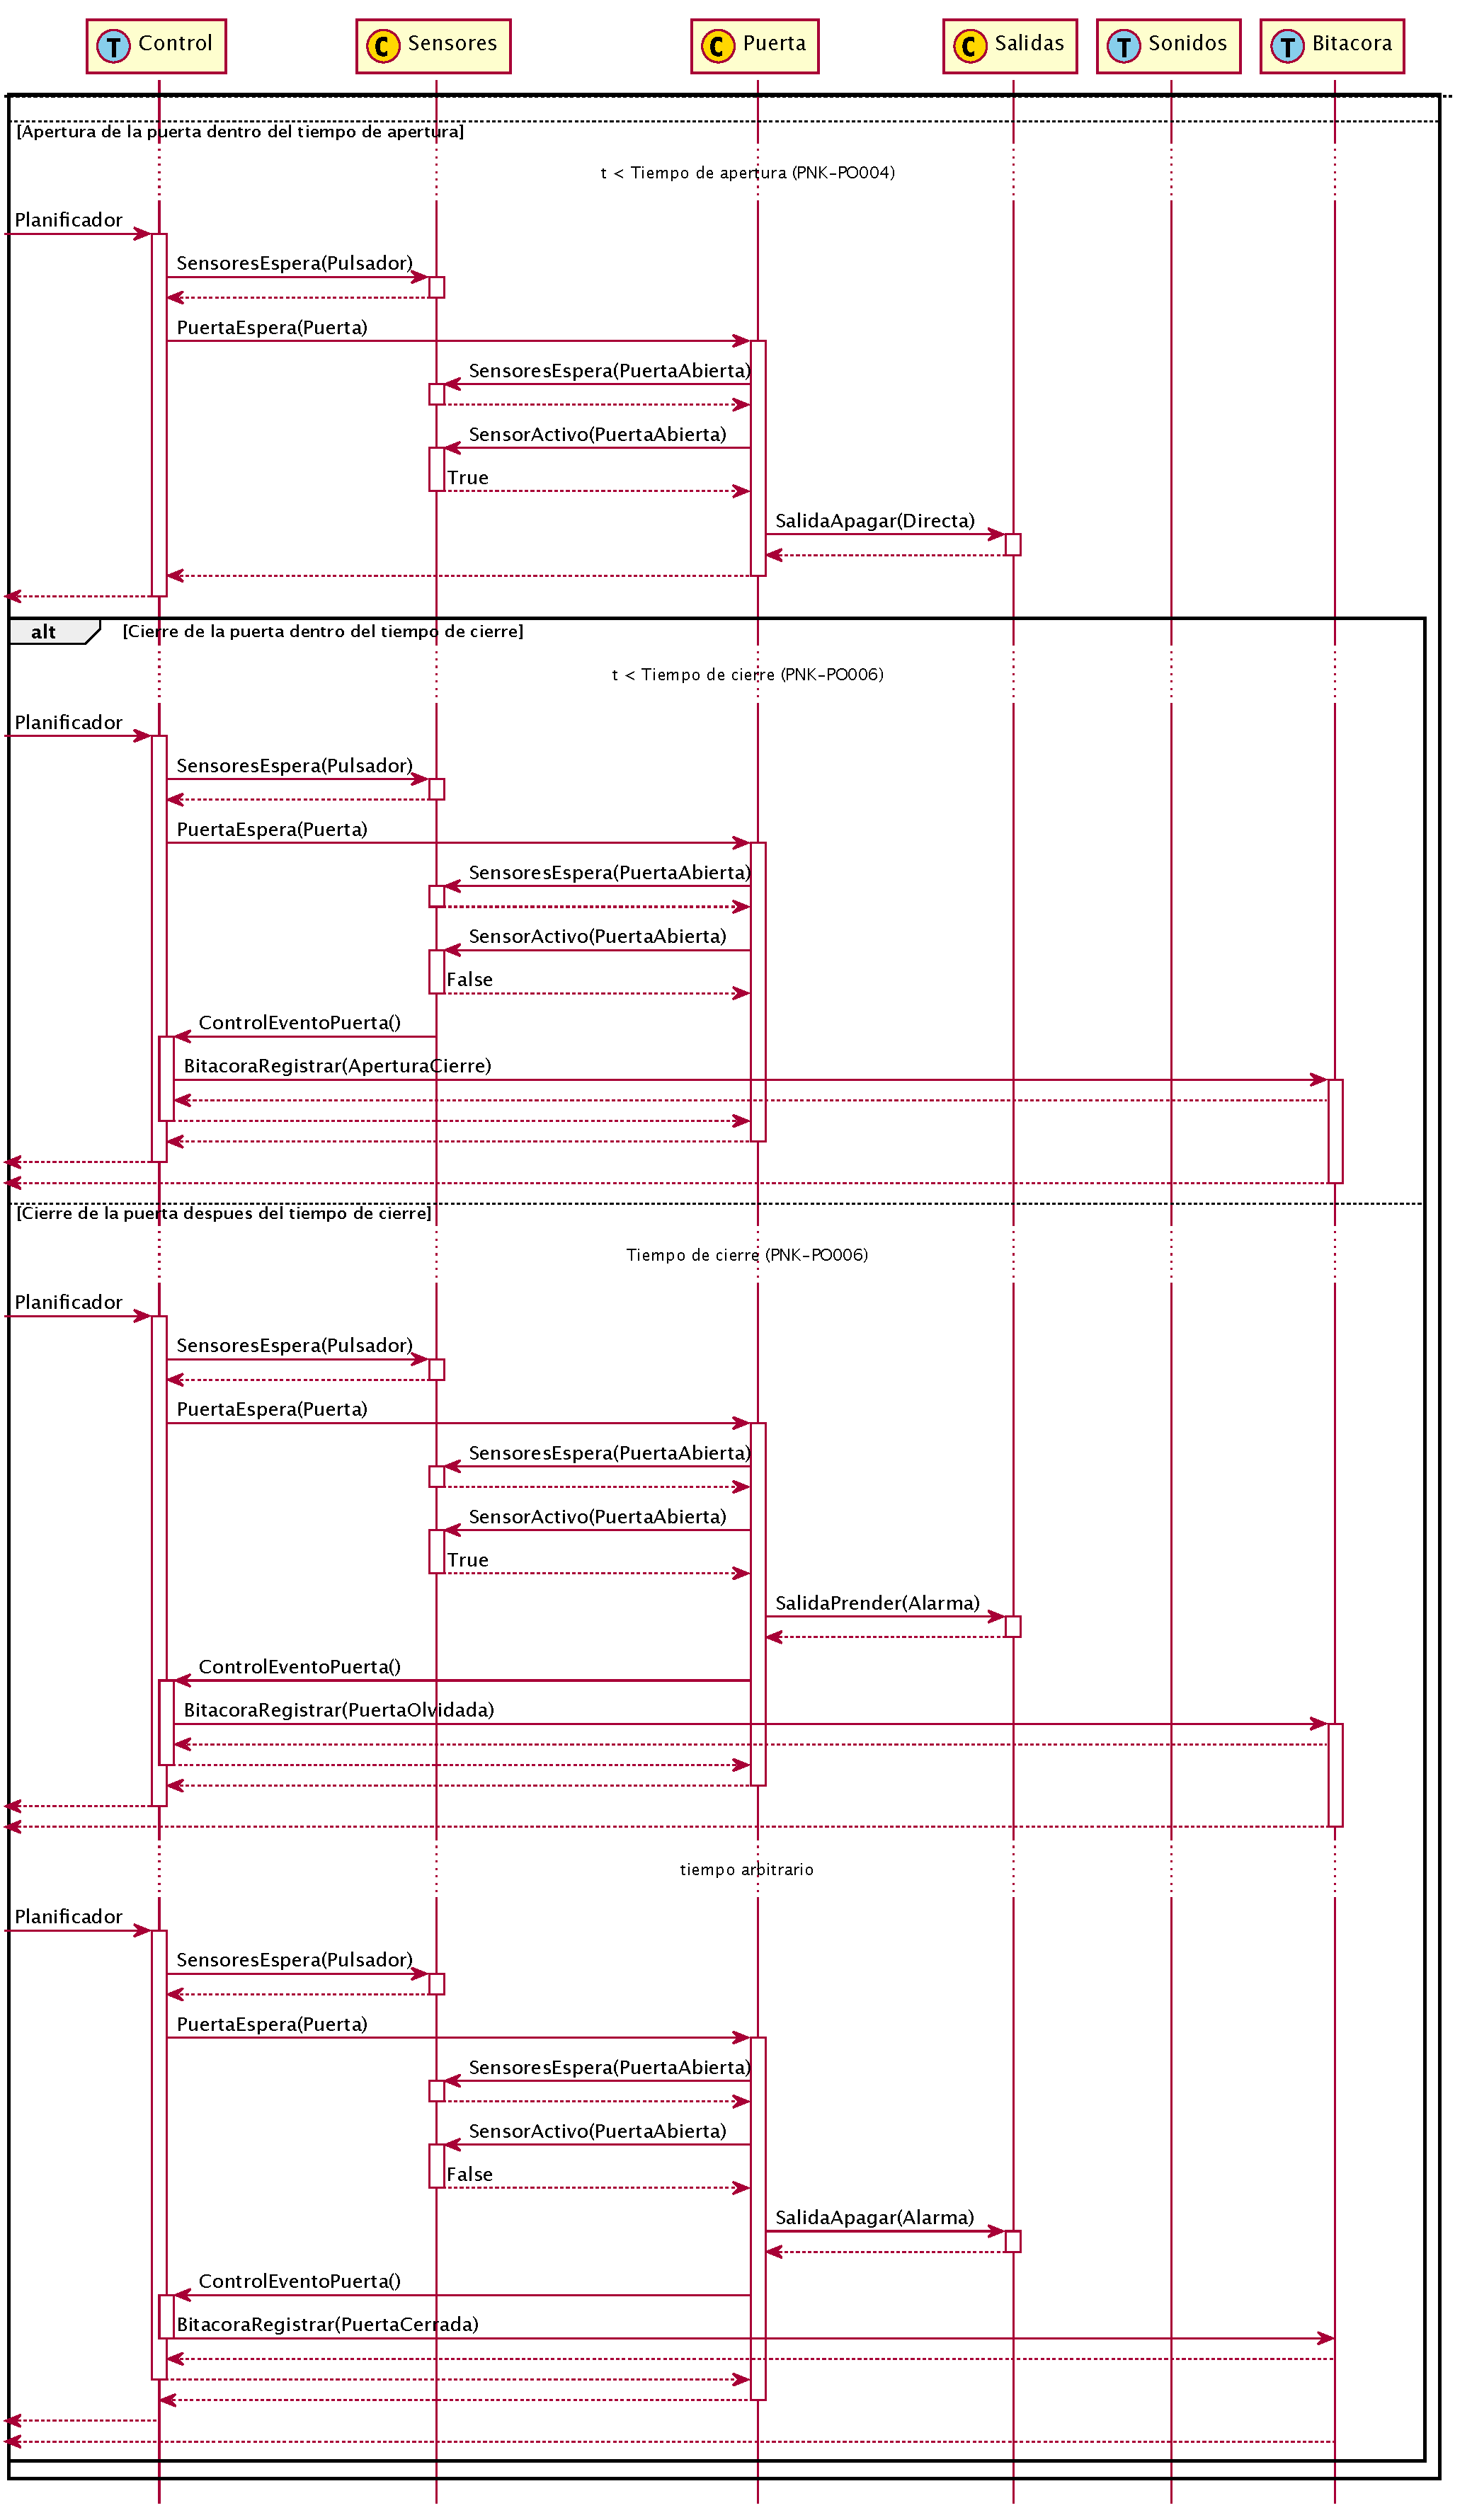
\includegraphics[width=\textwidth]{Figures/PNK-DS002-B.pdf}
	{\color{red} No es el diagrama correcto pero tiene la misma forma y extensión}
	\caption[Secuencia para el cambio de configuración]{Diagrama de secuencia para el cambio de configuración del equipo.}
	\label{fig:SecuenciaConfiguracion}
\end{figure}

\FloatBarrier

\section{Desarrollo del firmware}
\label{sec:desarrollo}

\subsection{Entorno de desarrollo}

Las metodologías de desarrollo propuestas por la ingeniería de software son lineamientos generales que deben ser ajustados a la realidad del equipo de desarrollo, y un proyecto que se inicia desde cero siempre es una buena oportunidad para adoptar nuevas metodologías. Por esta razón se decidió aplicar TDD (\emph{Test Driven Development}) para todo el proceso de codificación. Esta estrategia de trabajo plantea el desarrollo de una prueba unitaria que valida un requerimiento específico en primer lugar, y recién después el código de producción necesario para la implementación. Pero es un requisito indispensable disponer de una herramienta que compile y ejecute las pruebas unitarias en forma automática para poder implementar esta propuesta. La herramienta seleccionada para esta tarea fue Ceedling, un desarrollo en Ruby de código abierto pensado para implementar TDD en sistemas embebidos. Aunque realmente está formada por tres componentes que pueden ser utilizados en forma independiente, estos se acoplan perfectamente para funcionar como una solución integral. A estos se pueden sumar \emph{plugins}, propios o de terceros, que permiten agregar nuevas funcionalidades. Las componentes utilizadas en este trabajo fueron:

\begin{itemize}
	\item Unity: provee una variedad de funciones para verificar los resultados esperados en las pruebas unitarias. Estas funciones pueden comparar diferentes tipos de datos, e informan las discrepancias cuando los valores no son los correctos.

	\item Fake Function Framework: provee la capacidad de generar funciones Mock o Stub que permiten reemplazar las dependencias para poder implementar pruebas unitarias en clases que requieren código que no se desea probar.
	
	\item Ceedling: provee la compilación, ejecución y consolidación de los resultados de las pruebas unitarias, en forma automática y con un mínimo esfuerzo de configuración.
	
	\item GCOV: provee métricas con la cobertura de las pruebas ejecutadas, es decir la proporción de líneas de código fuente o de condiciones lógicas que fueron verificadas al ejecutar las pruebas unitarias.
	
	\item CLOC: provee métricas con la cantidad de comentarios y líneas de código fuente, para generar estadísticas que determinen la calidad del código.  
\end{itemize}

Otro de los aspectos que se buscó optimizar desde el inicio del proyecto fue la documentación, tanto del diseño general como del código en sí mismo. Para esto se seleccionaron dos herramientas también de código abierto que tienen la capacidad de trabajar en conjunto como si fueran una sola. Para la documentación del código se utilizó Doxygen, una programa que tiene la capacidad de generar la documentación de una biblioteca a partir de comentarios especiales ubicados en el código fuente. Para la escritura de los documentos de diseño se decidió utilizar la sintaxis Markdown y procesarlos también con Doxygen para unificar en un solo sitio WEB toda la información del desarrollo. Para los diagramas UML se utilizó PlantUML, una herramienta también de código abierto que puede funcionar en conjunto con Doxygen, y que permite generar los diagramas a partir de descripciones textuales muy simples y rápidas.

Finalmente, como entorno de desarrollo integrado se decidió utilizar Visual Studio Code, un editor de código abierto desarrollado por Microsoft, que funciona en las plataformas de Windows, Linux y MacOS indistintamente. Tiene además una extensa biblioteca de \emph{plugins} que le permiten extender la funcionalidad básica. De esta forma fue posible agregarle el reconocimiento de la sintaxis en el lenguaje C en los comentarios Doxygen, en los documentos Markdown y en los diagramas PlantUML. También se pudo disponer del procesamiento las advertencias por errores en la documentación devueltos por Doxygen, de la visualización de los diagramas UML generados por PlantUML, de la ejecución de las pruebas unitarias mediente Ceedling y de la gestión del repositorio GIT que almacenó el código. A estas herramientas debemos agregarles el ESP-IDF (\emph{Espressif IoT Development Framework}), el conjunto de bibliotecas y utilidades provistas por el fabricante del procesador para el desarrollo del software para los procesadores ESP32. De esta forma queda completo el entorno de desarrollo utilizado para el presente trabajo. En la tabla \ref{tab:HerramientasDesarrollo} se puede ver un resumen con el nombre de cada herramienta y una breve descripción de la función.

\begin{table}[ht]
	\centering
	\caption[Herramientas utilizadas para el desarrollo del firmware]{Resumen de herramientas utilizadas en el desarrollo del firmware del presente trabajo.}
	\begin{tabular}{L{25mm} L{100mm}}    
		\toprule
		\textbf{Nombre} & 
		\textbf{Funcionalidad proporcionada} \\
		\midrule
		Unity & 
		Verificación de los resultados en las pruebas unitarias y reporte de las discrepancias \\
		Fake Function Framework &
		Generación automática de funciones Mock y Stub para resolver las dependencias en las pruebas unitarias \\
		Ceedling &
		Resolución automáticamente de dependencias, compilación, ejecución y consolidación los resultados de las pruebas unitarias \\
		GCOV &
		Determinación de la cobertura en las pruebas unitarias y generación de un reporte en forma de página WEB \\
		CLOC &
		Generación de estadísticas con la proporción de comentarios y pruebas por línea de código fuente \\
		Doxygen &
		Generación de la documentación consolidada con la información del diseño y del código en forma de una página WEB \\
		PlantUML &
		Generación los diagramas UML a partir de descripciones textuales \\
		GIT &
		Mantenimiento de las versiones del código fuente del firmware, de la documentación de diseño y de los diagramas UML \\
		ESP-IDF &
		Biblioteca con los controladores y las herramientas de desarrollo provistas por el fabricante de la plataforma \\
		Visual Studio Code &
		Entorno de desarrollo integrado para la edición el código fuente y el manejo centralizado de las herramientas utilizadas en el proyecto \\
		\bottomrule
		\hline
	\end{tabular}
	\label{tab:HerramientasDesarrollo}
\end{table}

\subsection{Pruebas de integración en las tareas del sistema}

La plataforma de desarrollo provista por el fabricante utiliza a FreeRTOS como sistema operativo de tiempo real, donde se ejecutan como tareas los servicios de comunicaciones como el protocolo TCP/IP y el servidor HTTP. Esta versión de FreeRTOS ha sido modificada por el fabricante para poder ejecutarse en un procesador de doble núcleo como es ESP32. Por estas razones, utilizar otro sistema operativo de tiempo real implicaría un esfuerzo de desarrollo muy importante, que excedería ampliamente los alcances del presente trabajo. 

Lamentablemente FreeRTOS es un desarrollo complejo, que además de estar modularizado para facilitar la portación a diferentes arquitecturas, tiene un código que puede personalizarse utilizando el archivo FreeRTOSConfig.h. Todo esto hacen que sea imposible generar automáticamente funciones Stub o Mock que permitan implementar pruebas unitarias automatizadas en código que utiliza los servicios del sistema operativo. 

Una de las primeras estrategias para poder conciliar la idea de aplicar TDD con los problemas derivados de utilizar FreeRTOS fue dividir la aplicación en tres capas. De esta forma se buscó concentrar el código critico en los objetos de la capa de controladores, y como estos no utilizan los servicios del sistema operativo se pudieron desarrollar utilizando TDD. De todas formas esta solución no resultó totalmente satisfactoria, por lo que se siguió buscando una alternativa para poder ejecutar pruebas automatizadas sobre las tareas.

La solución definitiva a este problema se obtuvo combinando la portabilidad de FreeRTOS y la capacidad de Ceedling de utilizar \emph{plugins}. Para esto se desarrolló un \emph{plugin} propio que analiza el código fuente del archivo de prueba para determinar si utiliza los servicios del sistema operativo. En este caso modifica el proceso de compilación y enlazado para incluir una versión FreeRTOS que ejecuta como una tarea dentro de un ambiente POSIX. También modifica el código generado para el \emph{runner} de la prueba para iniciar el sistema operativo, y mueve la secuencia de pruebas a una tarea de FreeRTOS que detiene el planificador como ultima operación.

De esta forma, Ceedling puede generar un ejecutable que inicia el sistema operativo, ejecuta cada una de las pruebas en forma secuencial y termina una vez que se completaron las pruebas. Este comportamiento, que resulta natural en las pruebas automatizadas, es totalmente contrapuesto al uso normal de FreeRTOS, donde el sistema se inicia pero nunca se detiene. El resultado final de este desarrollo es la posibilidad de implementar pruebas automatizadas sobre las tareas de la capa de aplicación con las mismas herramientas utilizadas para el resto del desarrollo.

\subsection{Uso del tipo de abstracto de datos}

Como ya se mencionó en la subsección \ref{sub:Arquitectura}, para el modelado del firmware se utilizó una metodología orientada a objetos. Uno de los inconvenientes de aplicar esta propuesta es que el lenguaje C, el más utilizado en el desarrollo de sistemas embebidos, no es un lenguaje orientado a objetos.

Para resolver este problema existe una propuesta denominada ADT (\emph{Abstract Data Type}) que, explotando el uso de punteros a estructuras, permite emular muy fácilmente una programación orientada a objetos, utilizando el lenguaje C estándar. Esta técnica considera un archivo de cabeceras (.h) como la interfaz pública de la clase y el archivo de código fuente (.c) como la implementación privada, y  plantea el siguiente patrón de programación:

\begin{enumerate}
	\item La declaración incompleta de una estructura de datos en el archivo de cabeceras, que define el nombre pero sin enumerar los miembros. La declaración de esta estructura se realiza en forma completa en el archivo de código, y cada uno de sus campos es equivalente a un atributo privado del objeto.
	
	\item La declaración de un puntero a esta estructura también en el archivo de cabeceras. Este tipo de puntero podrá ser utilizado desde cualquier parte del proyecto, siempre que no se intente acceder al contenido de memoria referenciado. Esto permite encapsular los atributos del objeto y evitar que puedan ser alterados en forma externa.
	 
	\item Una o más funciones que devuelven como resultado un puntero a la estructura declarado en el apartado anterior. Estas funciones son el equivalente a los constructores de la clase, y además son responsables de la alocación del espacio de memoria necesario para almacenar la nueva instancia del objeto. Esta alocación podrá ser dinámica, y utilizar funciones como \emph{malloc}, o estática mediante un arreglo de estructuras.
	
	\item Varias funciones que reciben como primer parámetro el puntero retornado por las funciones constructoras, y que son equivalentes a los métodos públicos de la clase. 
\end{enumerate}

Este patrón de programación permite generar un código que puede escalar muy fácilmente, ya que resulta irrelevante la cantidad de instancias de un mismo elemento. De esta forma, a pesar de que el software desarrollado solo puede controlar una puerta, puede inmediatamente funcionar con dos o más puertas con solo efectuar dos llamadas al constructor de la clase Puerta. En las siguientes fracciones de código puede verse un ejemplo simplificado del patrón de programación descrito.

\begin{lstlisting}[caption=Porción simplificada del archivo de cabecera con la interfaz publica de la clase Puerta.] 
/* === Declaraciones de tipos de datos ====================== */
//! Tipo de datos para referenciar a un objeto puerta
typedef struct puerta_s * puerta_t;

/* === Declaraciones de funciones externas ================== */
//! Función para instanciar un objeto puerta
puerta_t PuertaCrear(void);

//! Función para configurar una puerta
bool PuertaConfigurar(puerta_t puerta, tiempo_t apertura);

//! Función para liberar la puerta y permitir un ingreso
void PuertaLiberar(puerta_t puerta);
\end{lstlisting}

\begin{lstlisting}[caption=Porción simplificada del archivo de código fuente con la implementación de la clase Puerta.] 
/* === Definicion y Macros ================================== */
//! Cantidad maxima de puertas alocadas estaticamente
#define PUERTAS_CANTIDAD                1

/* === Declaraciones de tipos de datos ====================== */
//! Estructura que describe la información de una puerta
struct puerta_s {
    puerta_estado_t estado;
    tiempo_t apertura;
    tiempo_t espera;
};

/* === Definiciones de funciones internas =================== */
//! Aloca la memoria necesaria para un nuevo objeto puerta
static puerta_t CrearInstancia(void) {
    puerta_t resultado = NULL;

    static int usadas = 0;
    static struct puerta_s puertas[PUERTAS_CANTIDAD] = {0};
    
    if (usadas < sizeof(puertas) / sizeof(struct puerta_s)) {
        memset(&puertas[usadas], 0, sizeof(struct puerta_s));
        resultado = &puertas[usadas];
        usadas++;
    }
    return resultado;
}

/* === Definiciones de funciones externas =================== */
puerta_t PuertaCrear(void) {
    puerta_t self = CrearInstancia();

    if (self != NULL) {
        self->estado = PUERTA_CERRADA;
        self->espera = 0;
    }
    return self;
}

bool PuertaConfigurar(puerta_t self, tiempo_t apertura) {
    bool resultado = false;

    if (self != NULL) {
        self->apertura = apertura;
        resultado = true;
    }
    return resultado;
}

void PuertaLiberar(puerta_t self) {
    if (self != NULL) {
        if (self->estado == PUERTA_CERRADA) {
            self->espera = self->apertura - 1;
            self->estado = PUERTA_LIBERADA;
        }
    }
}

\end{lstlisting}



% Chapter Template

\chapter{Ensayos y Resultados} % Main chapter title
\label{Chapter4}

Párrafo introductorio.

\section{Pruebas funcionales del hardware}
\label{sec:pruebasHW}

\section{Prototipo del hardware}
\label{sec:PruebasPrototipo}

Mediciones y verificaciones en el prototipo, se detallan las mediciones y ensayos realizados sobre la placa del prototipo para determinar su correcto funcionamiento

Correcciones en el prototipo: Se detallan los errores encontrados en el diseño y las correcciones efectuadas a partir de los ensayos funcionales en la placa del prototipo"

\begin{figure}[ht]
	\centering
	%	\includegraphics[scale=.3]{./Figures/cuadradoAzul.png}
	\caption{Imagen con el error en la definición del encapsulado del reloj de tiempo real}
	\label{fig:ErrorEncapsulado}
\end{figure}

\begin{figure}[ht]
	\centering
	%	\includegraphics[scale=.3]{./Figures/cuadradoAzul.png}
	\caption{Imagen con la corrección efectuada en la placa de prototipo}
	\label{fig:ImagenCorreccion}
\end{figure}

\section{Pruebas en el firmware}
\label{sec:PruebasFirmware}

\subsection{Pruebas unitarias}

Se describen las pruebas unitarias implementadas y los resultados obtenidos

\subsection{Pruebas de integración}

Se describen las pruebas de integración implementadas y los resultados obtenidos

\subsection{Resultados de las pruebas de aceptación del equipo}

Se analizan los resultados obtenidos al ejecutar las pruebas de aceptación definidas al inicio del proyecto

\section{Resultados}
\label{sec:Resultados}

Métricas del firmware desarrollado: se presentan métricas para evaluar la calidad del software desarrollado

\begin{table}[h]
	\centering
	\caption{Tabla resumen con las métricas de calidad obtenidas para el firmware desarrollado}
	\begin{tabular}{l c}    
		\toprule
		\textbf{Equipo} 	 & \textbf{Valor}\\
		\midrule
		Punku 				 & \$ 3.000\\
		\bottomrule
		\hline
	\end{tabular}
	\label{tab:MetricasFirmware}
\end{table}


Comparaciones con productos existentes: se repite la comparación de las prestaciones de los equipos existentes con el equipo anterior y con el nuevo equipo desarrollado en función de los resultados obtenidos

\begin{table}[h]
	\centering
	\caption{Cuadro comparativo del equipo actual con el anterior y con otros equipos del mercado}
	\begin{tabular}{l c}    
		\toprule
		\textbf{Equipo} 	 & \textbf{Valor}\\
		\midrule
		Punku 				 & \$ 3.000\\
		\bottomrule
		\hline
	\end{tabular}
	\label{tab:ComparacionNuevo}
\end{table}

Comparaciones de los riesgos planificados con el resultado del proyecto: se analizan los resultados obtenidos por las acciones destinadas a mitigar los riesgos identificados en la planificación del proyecto
 
\chapter{Conclusiones}
\label{Chapter5}

En el presente capítulo se resumen las conclusiones obtenidas al completar el trabajo y se presentan los posibles pasos a seguir.

\section{Resultados Obtenidos}

Si se contrastan los objetivos planteados en la sección \ref{sec:objetivos} con el desarrollo expuesto en capítulo \ref{Chapter3} se obtienen las siguientes conclusiones:

\begin{enumerate}
	\item El primer objetivo se cumplió, ya que el equipo desarrollado utiliza un microcontrolador ESP-32 que incorpora interfaces de comunicación WiFi y Bluetooth.
	
	\item El segundo objetivo también se cumplió, dado que el diseño actual incorpora un RTC con respaldo de batería, que le permite mantener la fecha y hora válidas aun cuando se produzcan interrupciones en el suministro de energía eléctrica.
	
	\item El nuevo equipo está diseñado para controlar indistintamente cerraduras electromagnéticas o motorizadas, por lo tanto el tercer objetivo también está cumplido.
	
	\item El nuevo equipo mantiene las características generales el diseño original, pero al utilizar una API REST sobre HTTP, resulta más simple de gestionar. Además gracias al cambio de procesador y a la unificación de las unidades funcionales, resulta más económico que el equipo original. Esto permite afirmar que el cuarto objetivo también está cumplido.
	
	\item El diseño y la codificación orientados a objetos utilizados para el desarrollo del firmware permite ampliar fácilmente las capacidades del equipo. Las pruebas automatizadas implementadas disminuyen la posibilidad de introducir errores al hacer cambios en el código. Todo esto constituye una plataforma modular que permite escalar las funcionalidades del equipo, por lo que se puede afirmar que también el quinto objetivo está cumplido.
\end{enumerate}

En la tabla \ref{tab:ComparacionActual} se repite el análisis de los equipos para control de acceso existentes en el mercado, incluyendo ahora al equipo desarrollado. Como puede observarse este último ofrece mayor cantidad de funcionalidades a un precio muy competitivo.

\begin{table}[H]
	\centering
	\caption{Cuadro comparativo con otros equipos del mercado}
	\begin{tabular}{C{25mm} C{25mm} C{50mm} C{20mm}}    
		\toprule
		\textbf{Equipo}  
		& \textbf{Tecnología} 
		& \textbf{Forma de gestión}
		& \textbf{Valor}  \\
		\midrule
		EQUISER \newline Punku (Original)
		& Proximidad y remotos RF
		& Gestionado desde un \newline celular usando Bluetooth
		& \$ 3.000\\
		\midrule
		Tebas \newline 208NW \cite{TEBAS}
		& Proximidad
		& Teclado numérico \newline integrado en el equipo
		& \$ 4.000\\
		\midrule
		ZK \newline MA300IS \cite{ZK}
		& Proximidad \newline y huellas
		& Computadora conectada \newline mediante Ethernet
		& \$ 10.000\\
		\midrule
		ANVIZ \newline T5 Pro \cite{ANVIZ}
		& Proximidad \newline y huellas
		& Computadora conectada \newline mediante Ethernet o USB
		& \$ 8.000\\
		\midrule
		EQUISER \newline Punku (Nuevo)
		& Proximidad (Mifare)
		& Gestionado desde un celular o una computadora \newline usando WiFi o Internet
		& \$ 3.000\\
		\bottomrule
		
		\hline
	\end{tabular}
	\label{tab:ComparacionActual}
\end{table}

Estos resultados permiten afirmar que el equipo desarrollado cumple con todos los objetivos planteados, y que brinda a la empresa EQUISER una nueva opción más competitiva para participar en el mercado de los sistemas para control de accesos. El esfuerzo invertido, principalmente en el desarrollo del firmware, generó una plataforma confiable y flexible que permite, además, ampliar esta oferta en un futuro con muy poco esfuerzo.

\section{Trabajo Futuro}

En lo que respecta al equipo desarrollado el próximo paso es, naturalmente, la fabricación de un segundo prototipo de la placa electrónica que incluya todas las correcciones efectuadas como parte de este trabajo. Este equipo debería ser sometido a pruebas de campo con clientes reales para validar el correcto funcionamiento en las condiciones normales de operación.

También es imprescindible el desarrollo de un software de gestión para dispositivos móviles que permita al cliente final operar con el equipo. La versión actual de Punku se gestiona con un software desarrollado en Java que solo funciona en dispositivos Android, la intención es reemplazarlo por una aplicación híbrida que pueda ejecutarse tanto en iOS con en Android, utilizando el mismo código. 

Desde el punto de vista académico se plantea también un trabajo derivado que puede resultar muy interesante: la automatización total de las pruebas del equipo. En este sentido el \emph{plugin} desarrollado para permitir la ejecución automatizada de las pruebas de integración que utilizan FreeRTOS es un paso importante, pero que no se pudo explotar completamente por falta de tiempo. Un desafío interesante es aplicar los conceptos de integración continua en este proyecto, incluyendo las pruebas de aceptación que involucran el uso de hardware especifico para simular la iteración de los usuarios con el equipo.
 

%----------------------------------------------------------------------------------------
%	CONTENIDO DE LA MEMORIA  - APÉNDICES
%----------------------------------------------------------------------------------------

\appendix % indicativo para indicarle a LaTeX los siguientes "capítulos" son apéndices

% Incluir los apéndices de la memoria como archivos separadas desde la carpeta Appendices
% Descomentar las líneas a medida que se escriben los apéndices

%\include{Appendices/AppendixA}
%\include{Appendices/AppendixB}
%\include{Appendices/AppendixC}

%----------------------------------------------------------------------------------------
%	BIBLIOGRAPHY
%----------------------------------------------------------------------------------------

\Urlmuskip=0mu plus 1mu\relax
\raggedright
\printbibliography[heading=bibintoc]

%----------------------------------------------------------------------------------------

\end{document}  
